\section{$\pi^0$ data-MC}
\label{app:pi0}
\par Data shown passing the $\pi^0$ filter refers to two separate selections. The first is a set of loose cuts implemented to develop a $\pi^0$ filter run through production which meets MicroBooNE's blindness requirements. Data-MC comparisons of the input variables for these selections are shown in sec.~\ref{app:pi0:input}. The selection cuts applied are:
\begin{itemize}
    \item One reconstructed neutrino slice in the event: \texttt{nslice} $=$ 1.
    \item Both shower candidates must have a track-score (variable \texttt{pi0\_shrscore\_1,2}) $<$ 0.8.
    \item Shower direction aligned with vertex-shower start direction: \texttt{pi0\_dot\_1,2} $>$ 0.8.
    \item Conversion distance (\texttt{pi0\_radlen\_1,2}) greater than 3 cm.
    \item Dot product between opening angle between the two showers (\texttt{pi0\_gammadot}) $<$ 0.94.
    \item Leading shower collection-plane energy (\texttt{pi0\_energy1\_Y}) $>$ 50 MeV.
    \item Sub-leading shower collection-plane energy (\texttt{pi0\_energy2\_Y}) $>$ 20 MeV.
\end{itemize}
For comparisons of physics quantities comparisons are made after a tighter, more $\pi^0$ pure selection. These cuts are applied to produce the comparisons for $\pi^0$ kinematics (sec.~\ref{app:pi0:kinematics}), $\pi^0$ calorimetric variables (sec.~\ref{app:pi0:calorimetry}), and $\nu_e$ input variables (sec.~\ref{app:pi0:nueselection}). The selection is defined below:
\begin{itemize}
    \item One reconstructed neutrino slice in the event: \texttt{nslice} $=$ 1.
    \item Both shower candidates must have a track-score (variable \texttt{pi0\_shrscore\_1,2}) $<$ 0.5.
    \item Shower direction aligned with vertex-shower start direction: \texttt{pi0\_dot\_1,2} $>$ 0.8.
    \item Conversion distance (\texttt{pi0\_radlen\_1,2}) greater than 3 cm.
    \item Dot product between opening angle between the two showers (\texttt{pi0\_gammadot}) $<$ 0.94.
    \item Leading shower collection-plane energy (\texttt{pi0\_energy1\_Y}) $>$ 60 MeV.
    \item Sub-leading shower collection-plane energy (\texttt{pi0\_energy2\_Y}) $>$ 40 MeV.
    \item d$E$/d$x$  of leading shower (\texttt{pi0\_dedx1\_fit\_Y}) $>$ 1 MeV/cm.
\end{itemize}
\par These comparisons are performed after a flat 0.759 scaling is applied to CC and NC $\pi^0$ events based on the normalization differences found in the $\pi^0$ mass distributions from this selection. This allows to perform-shape-only comparisons. Errors in this section are stats-only. This scaling is different from the energy-dependent $\pi^0$-``tune'' implemented in the analysis using input from a broader set of sidebands.


\subsection{$\pi^0$ filter}
\label{app:pi0:input}
\par Figures~\ref{fig:pi0:inputs:shrscore1:RUN1}-\ref{fig:pi0:inputs:dot2:RUN1} show the distribution of reconstructed quantities for inputs to the $\pi^0$ selection. 
\begin{figure}[H] 
\begin{center}
    \begin{subfigure}[b]{0.3\textwidth}
    \centering
    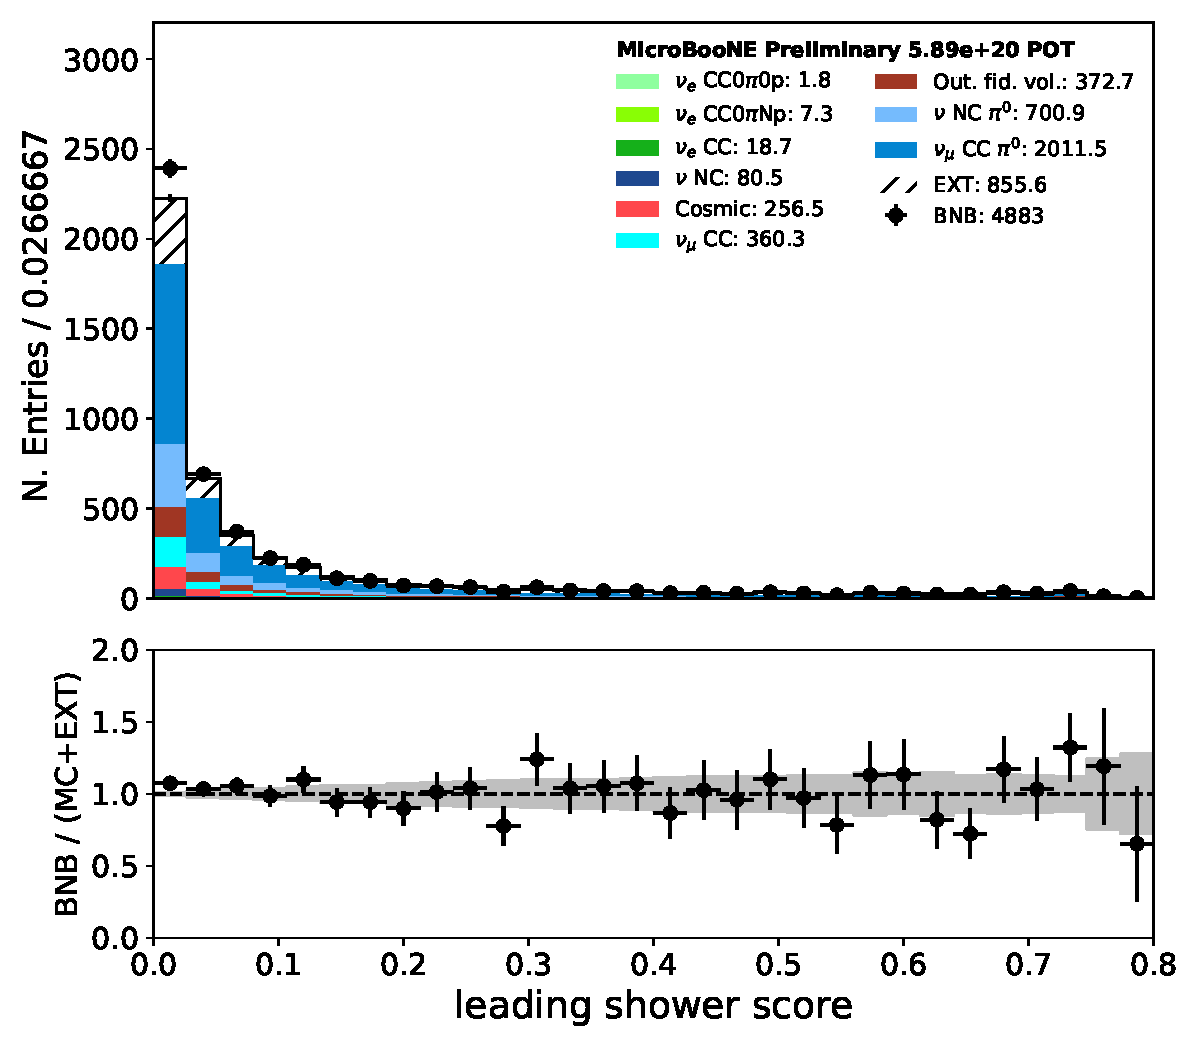
\includegraphics[width=1.00\textwidth]{pi0/inputs/pi0_shrscore1_03182020_presel.pdf}
    \caption{\label{fig:pi0:inputs:shrscore1:RUN1} pi0\_shrscore1}
    \end{subfigure}
    \begin{subfigure}[b]{0.3\textwidth}
    \centering
    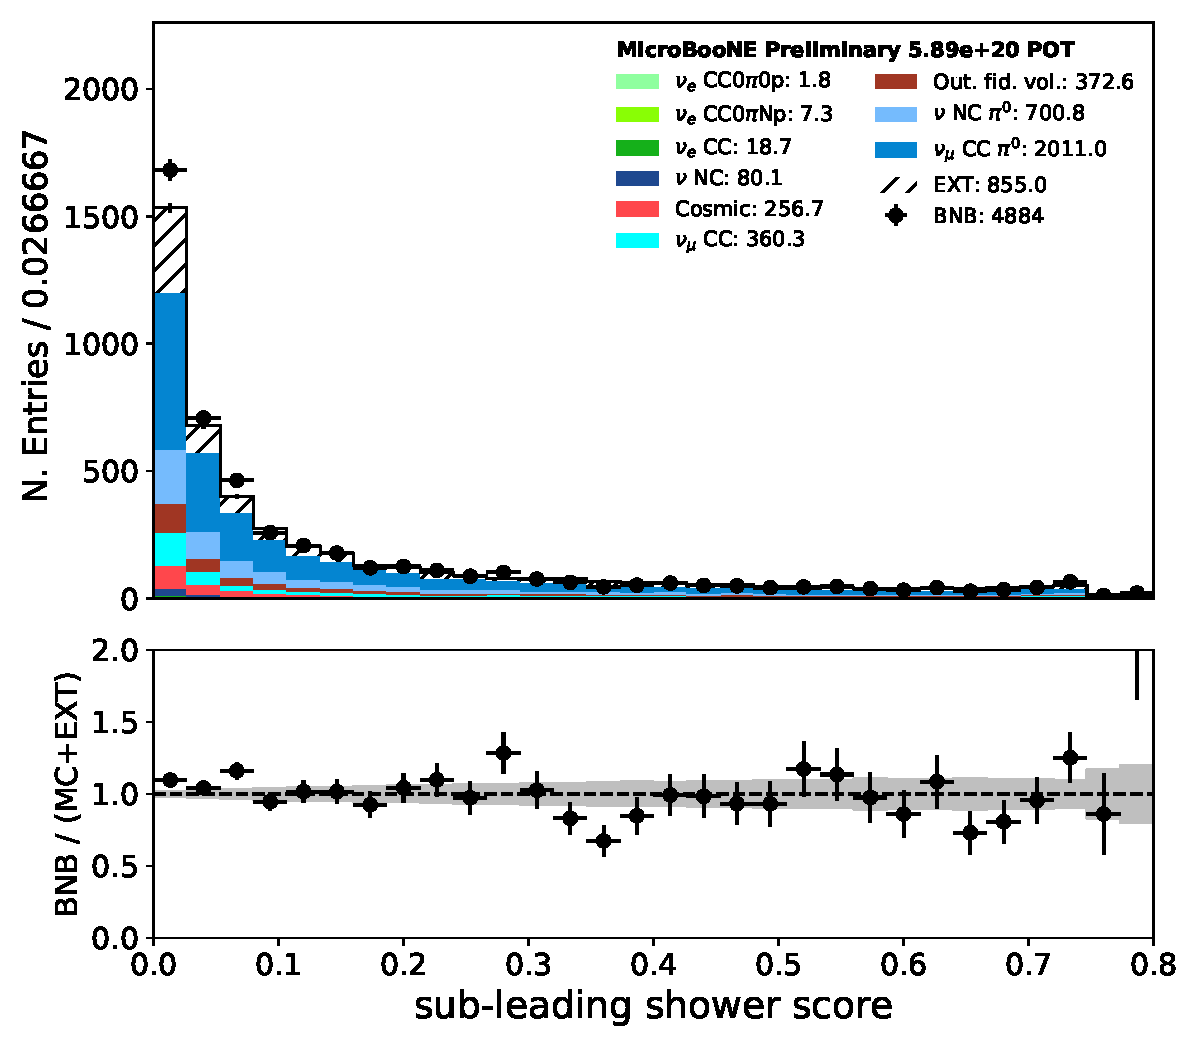
\includegraphics[width=1.00\textwidth]{pi0/inputs/pi0_shrscore2_03182020_presel.pdf}
    \caption{\label{fig:pi0:inputs:shrscore2:RUN1} pi0\_shrscore2}
    \end{subfigure}
    \begin{subfigure}[b]{0.3\textwidth}
    \centering
    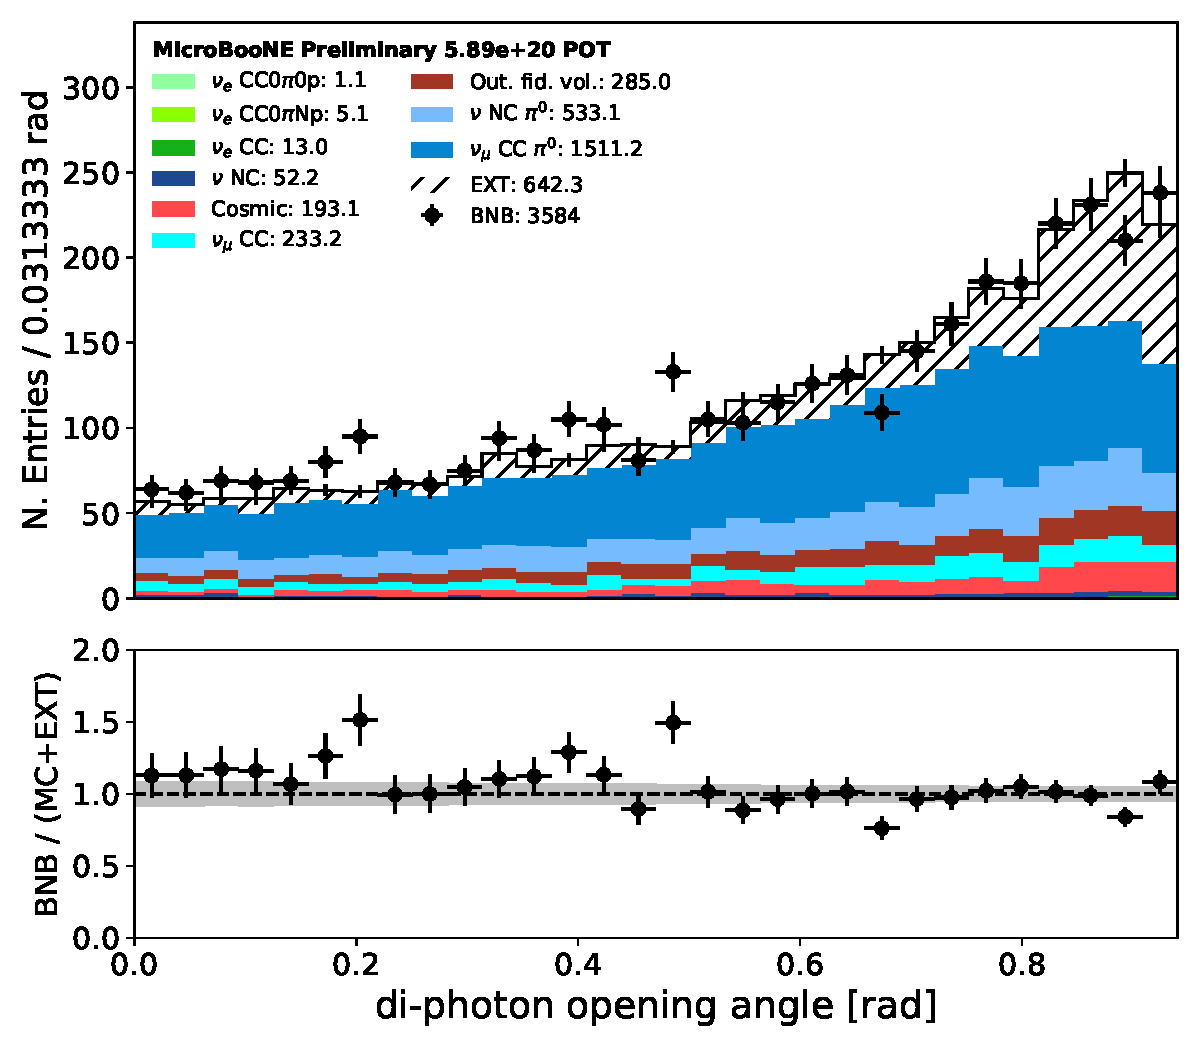
\includegraphics[width=1.00\textwidth]{pi0/inputs/pi0_gammadot_03182020_presel.pdf}
    \caption{\label{fig:pi0:inputs:gammadot:RUN1} pi0\_gammadot}
    \end{subfigure}
\end{center}
\end{figure}

\begin{figure}[H] 
\begin{center}
    \begin{subfigure}[b]{0.3\textwidth}
    \centering
    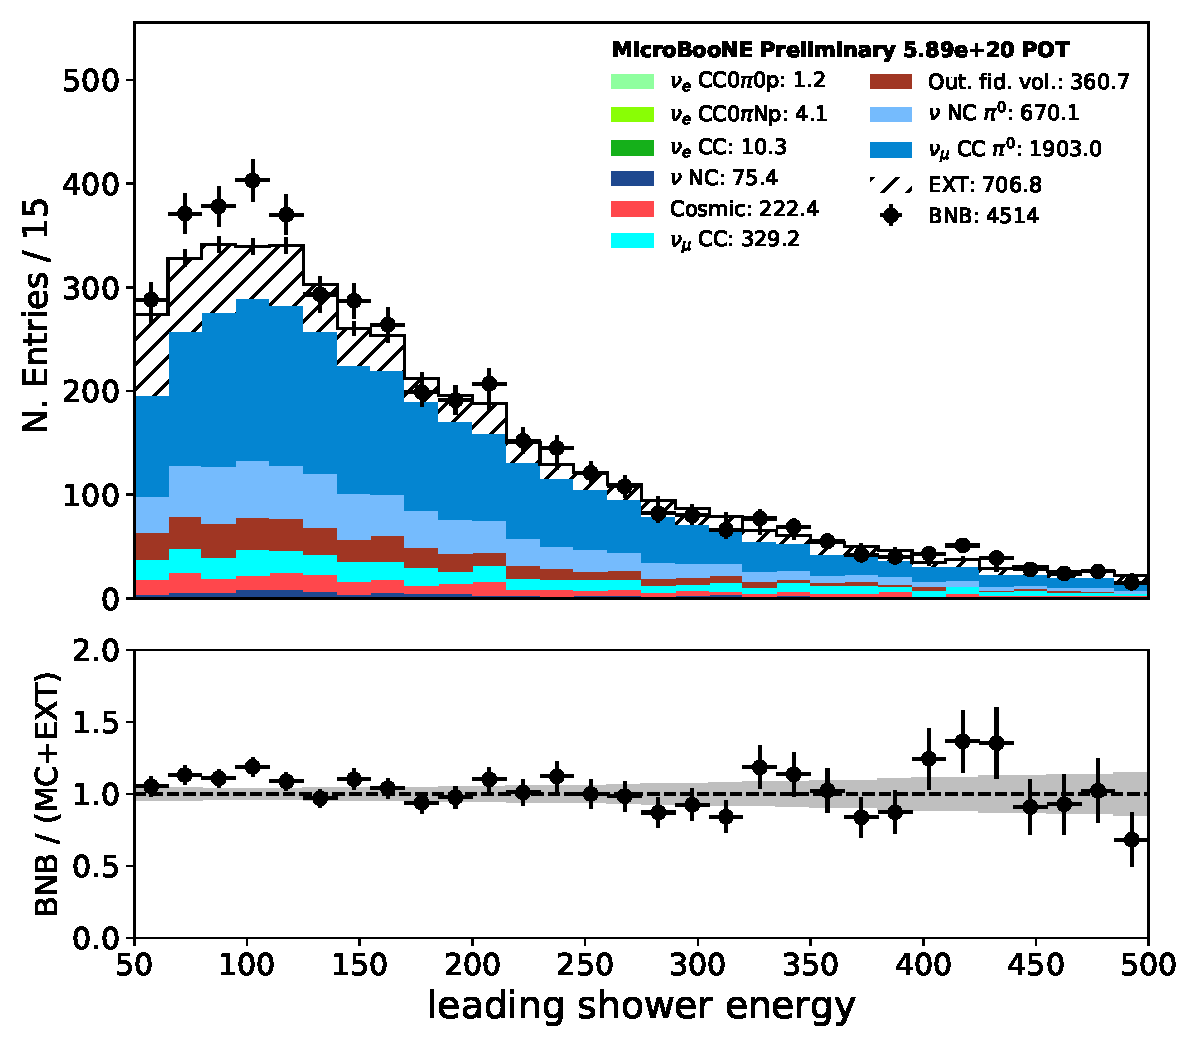
\includegraphics[width=1.00\textwidth]{pi0/inputs/pi0_energy1_Y_03182020_presel.pdf}
    \caption{\label{fig:pi0:inputs:energy1:RUN1} pi0\_energy1\_Y}
    \end{subfigure}
    \begin{subfigure}[b]{0.3\textwidth}
    \centering
    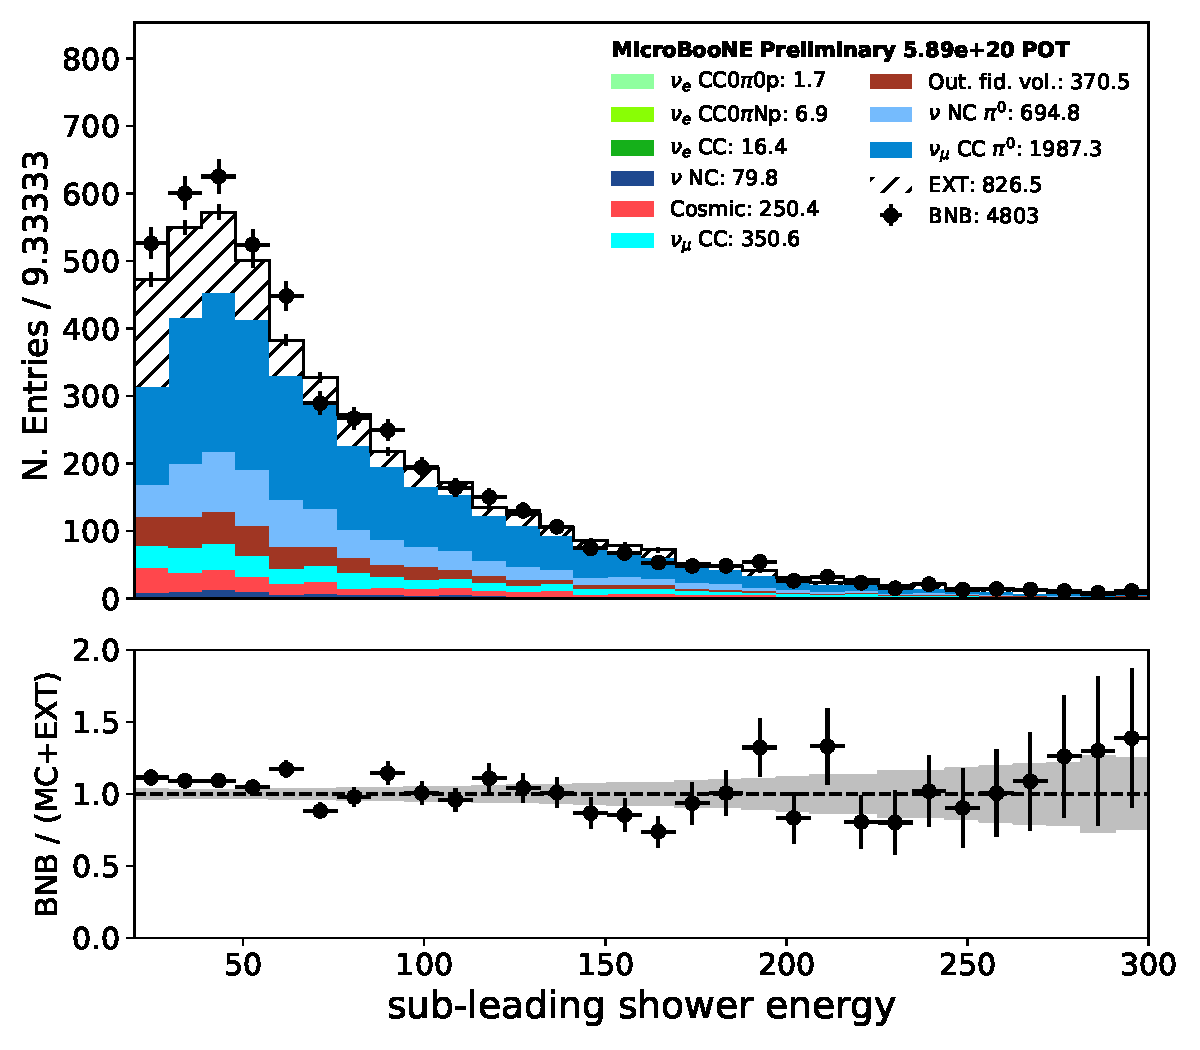
\includegraphics[width=1.00\textwidth]{pi0/inputs/pi0_energy2_Y_03182020_presel.pdf}
    \caption{\label{fig:pi0:inputs:energy12:RUN1} pi0\_energy2\_Y}
    \end{subfigure}
    \begin{subfigure}[b]{0.3\textwidth}
    \centering
    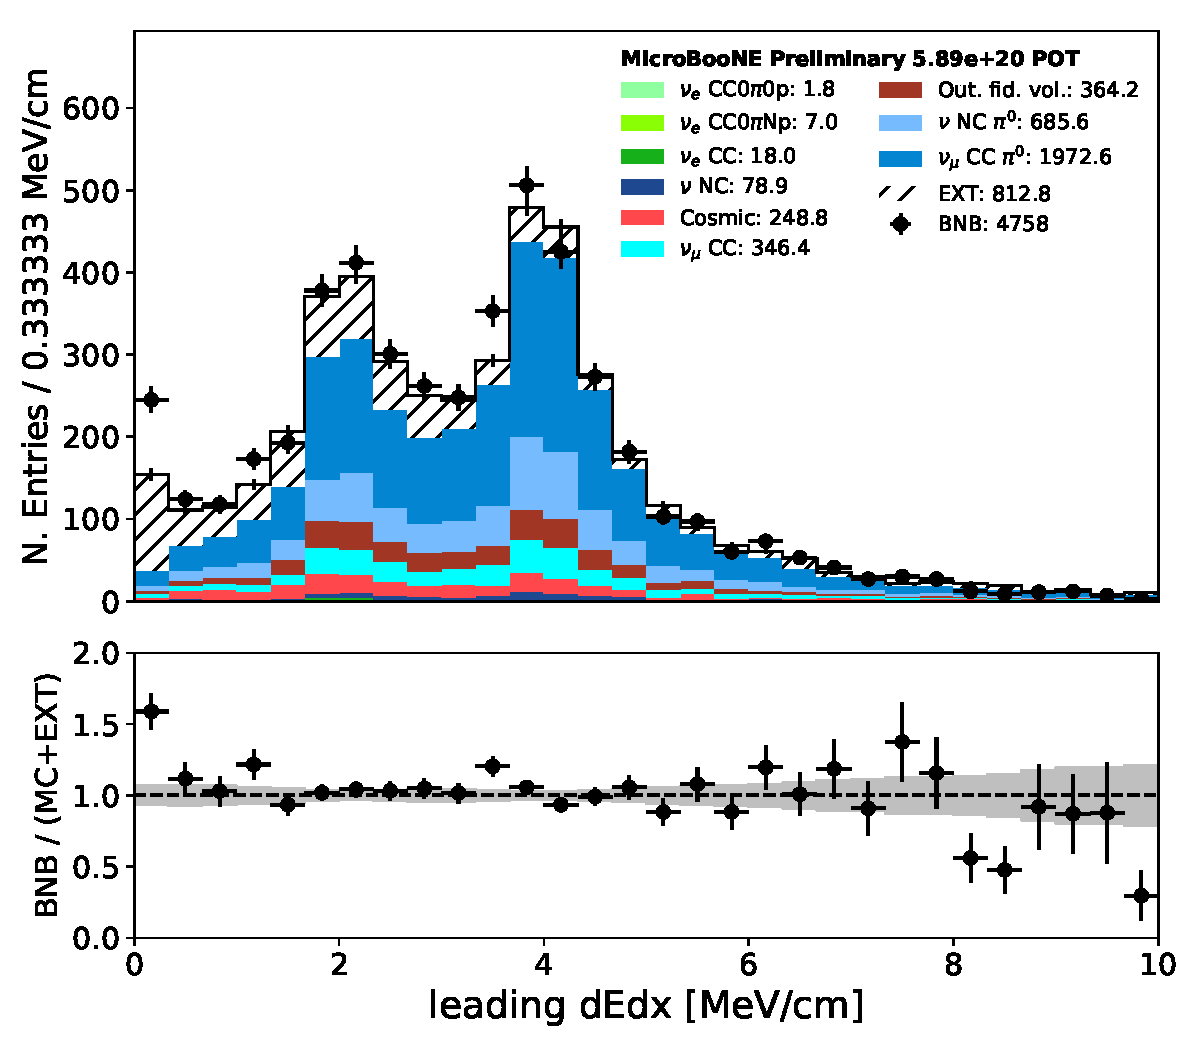
\includegraphics[width=1.00\textwidth]{pi0/inputs/pi0_dedx1_fit_Y_03182020_presel.pdf}
    \caption{\label{fig:pi0:inputs:gammadot:RUN1} pi0\_dedx1\_fit\_Y}
    \end{subfigure}
\end{center}
\end{figure}

\begin{figure}[H] 
\begin{center}
    \begin{subfigure}[b]{0.3\textwidth}
    \centering
    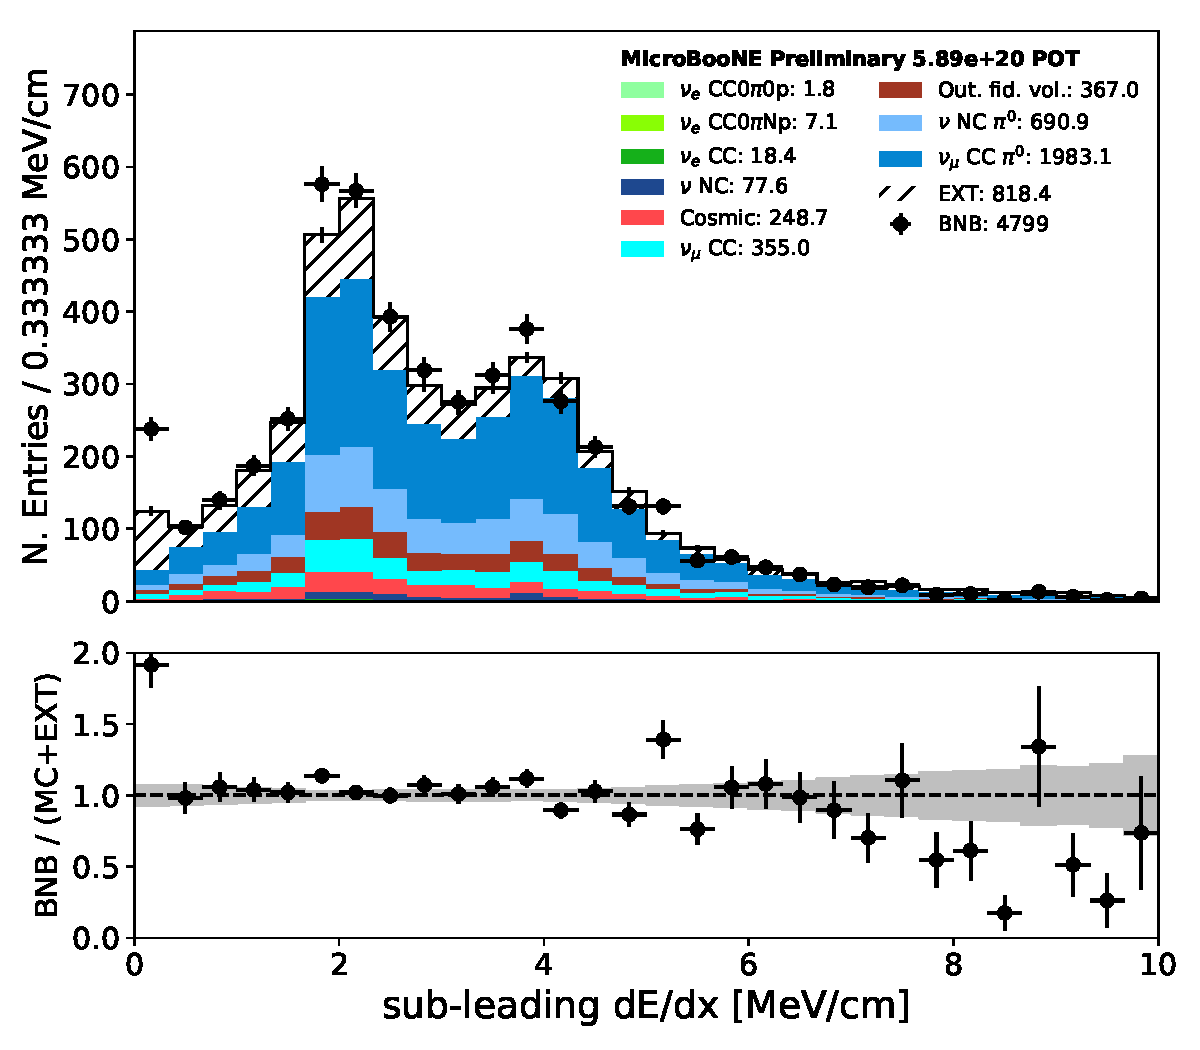
\includegraphics[width=1.00\textwidth]{pi0/inputs/pi0_dedx2_fit_Y_03182020_presel.pdf}
    \caption{\label{fig:pi0:inputs:dedx2:RUN1} pi0\_dedx2\_fit\_Y}
    \end{subfigure}
    \begin{subfigure}[b]{0.3\textwidth}
    \centering
    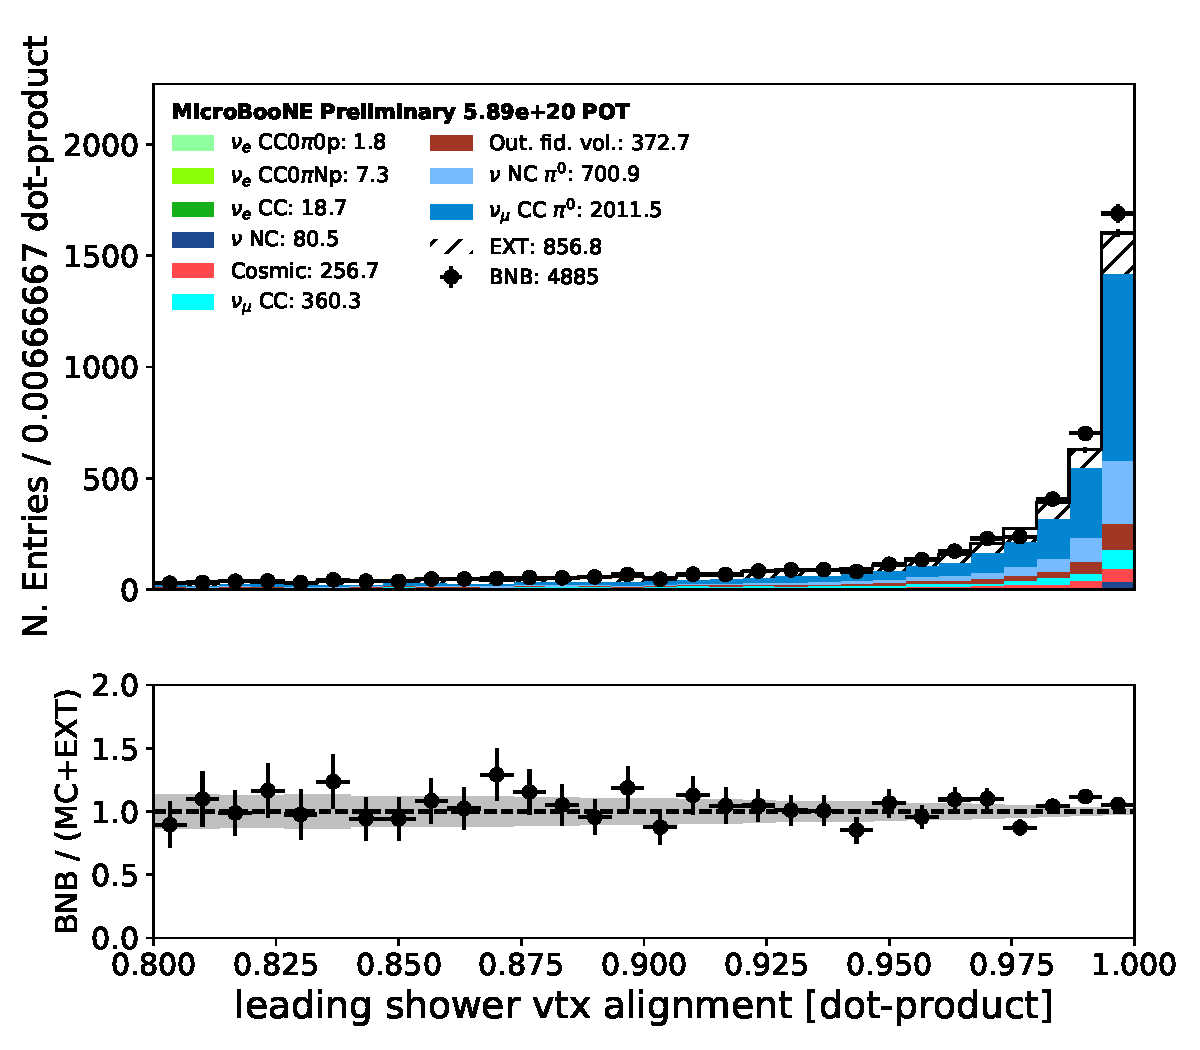
\includegraphics[width=1.00\textwidth]{pi0/inputs/pi0_dot1_03182020_presel.pdf}
    \caption{\label{fig:pi0:inputs:dot1:RUN1} pi0\_dot1}
    \end{subfigure}
    \begin{subfigure}[b]{0.3\textwidth}
    \centering
    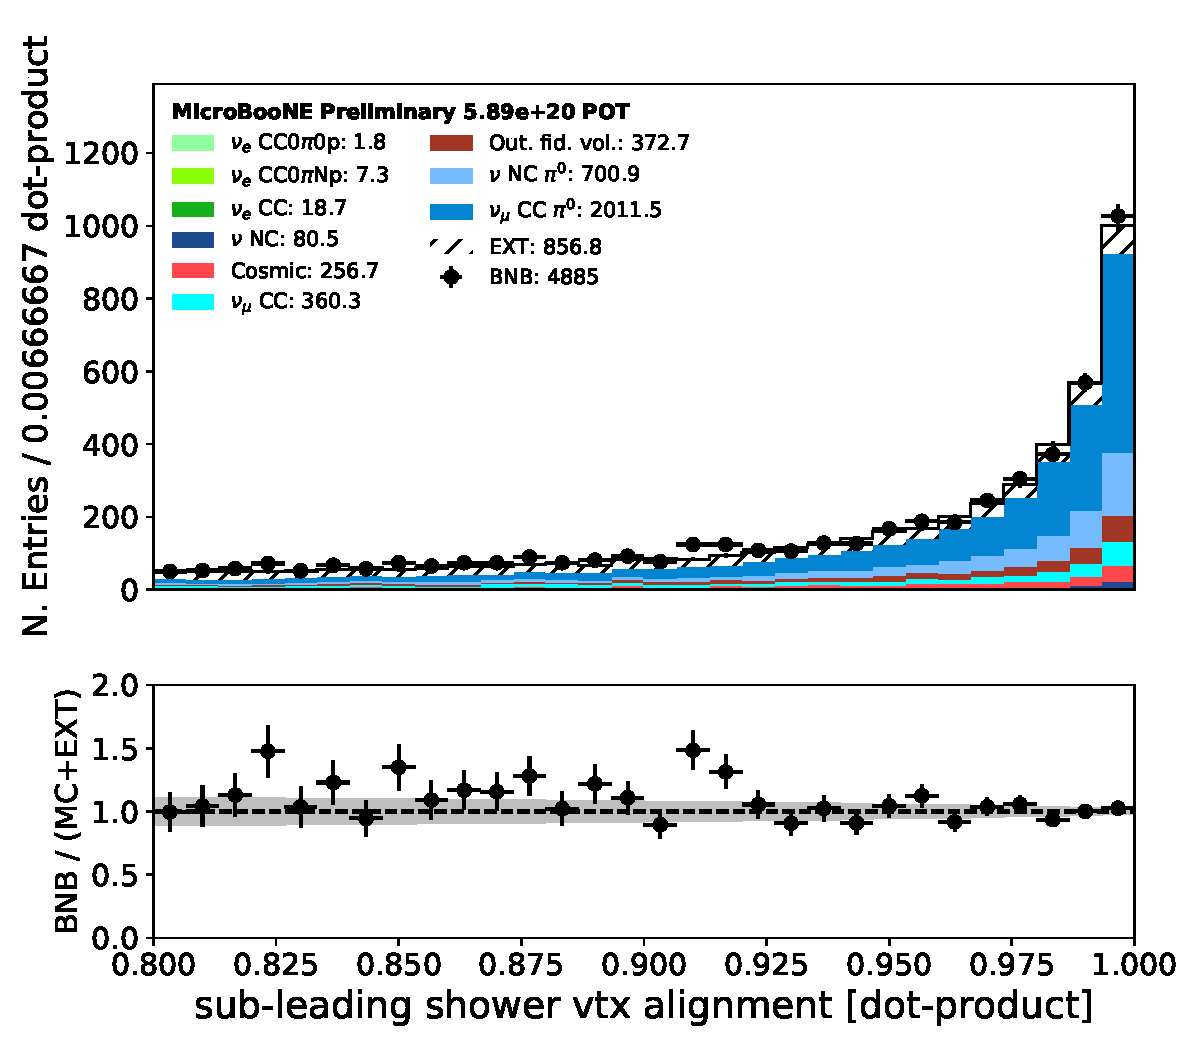
\includegraphics[width=1.00\textwidth]{pi0/inputs/pi0_dot2_03182020_presel.pdf}
    \caption{\label{fig:pi0:inputs:dot2:RUN1} pi0\_dot2}
    \end{subfigure}
\end{center}
\end{figure}

\begin{figure}[H] 
\begin{center}
    \begin{subfigure}[b]{0.3\textwidth}
    \centering
    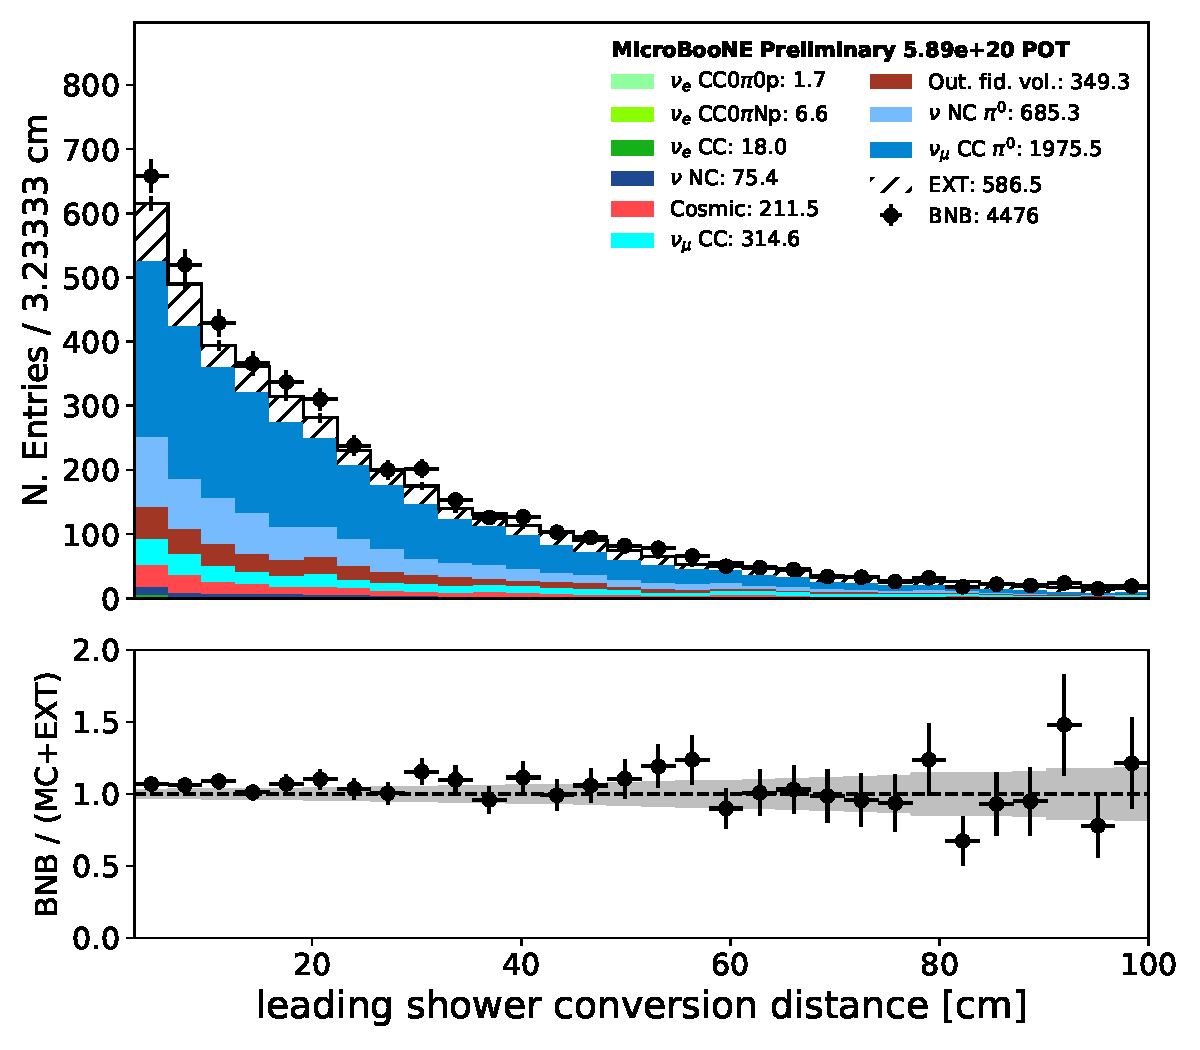
\includegraphics[width=1.00\textwidth]{pi0/inputs/pi0_radlen1_03182020_presel.pdf}
    \caption{\label{fig:pi0:inputs:radlen1:RUN1} pi0\_radlen1}
    \end{subfigure}
    \begin{subfigure}[b]{0.3\textwidth}
    \centering
    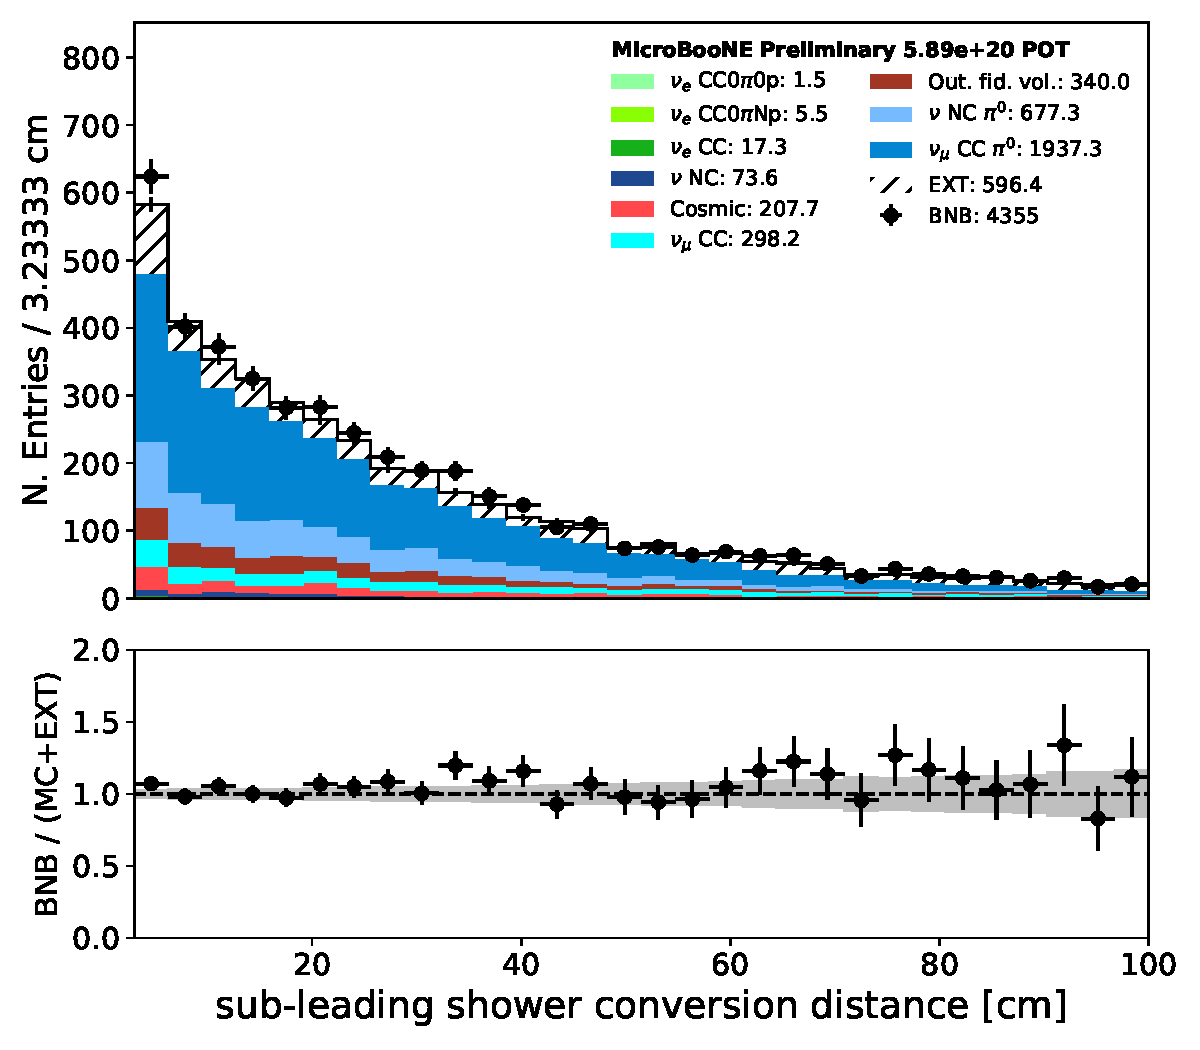
\includegraphics[width=1.00\textwidth]{pi0/inputs/pi0_radlen2_03182020_presel.pdf}
    \caption{\label{fig:pi0:inputs:radlen2:RUN1} pi0\_radlen2}
    \end{subfigure}
\end{center}
\end{figure}


\subsection{$\pi^0$ kinematics}
\label{app:pi0:kinematics}

\begin{figure}[H] 
\begin{center}
    \begin{subfigure}[b]{0.3\textwidth}
    \centering
    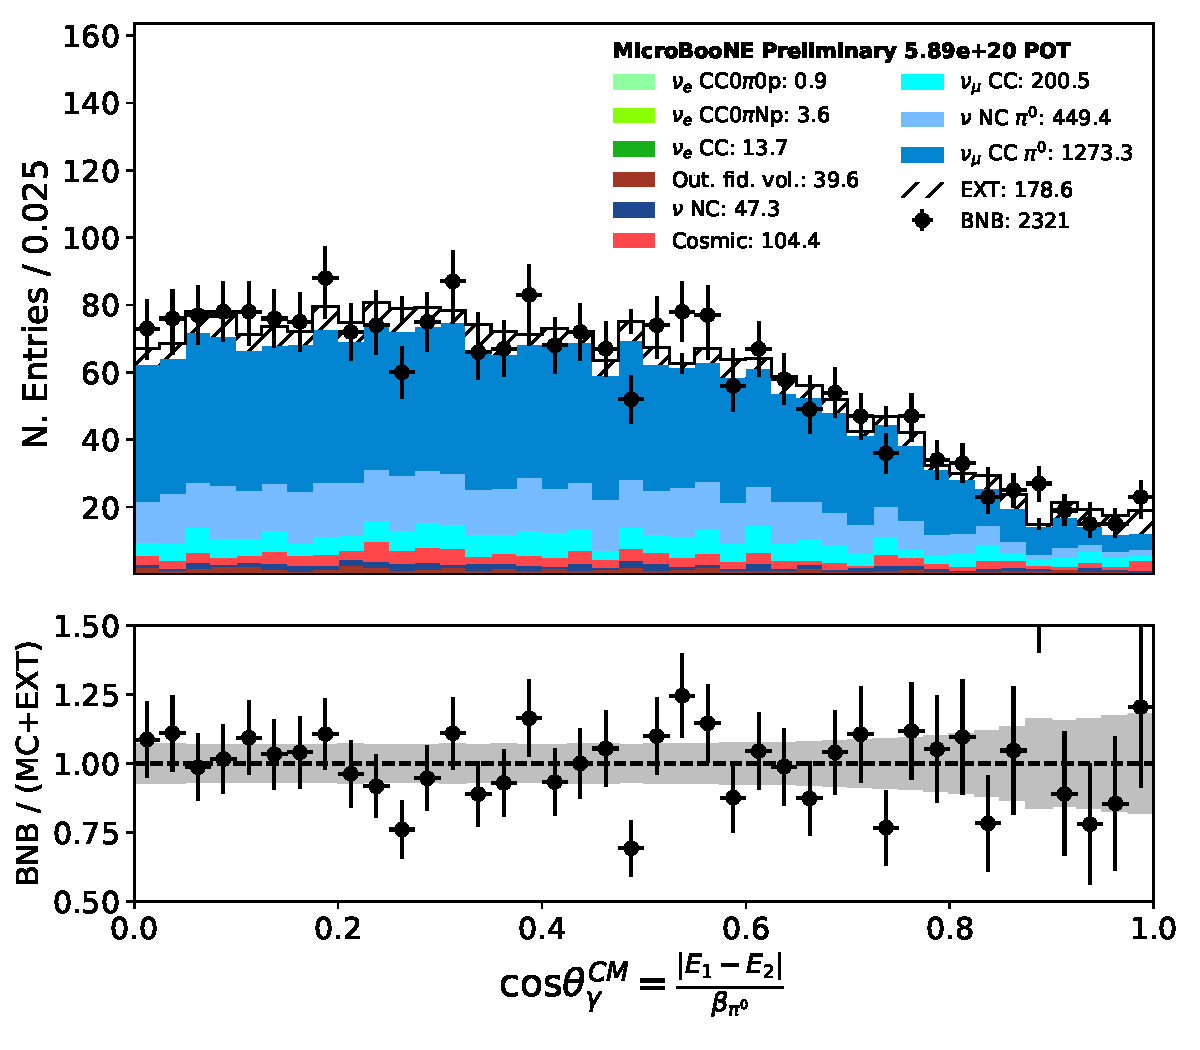
\includegraphics[width=1.00\textwidth]{pi0/kinematics/pi0thetacm_03112020_ALL_scaled.pdf}
    \caption{}
    \end{subfigure}
    \begin{subfigure}[b]{0.3\textwidth}
    \centering
    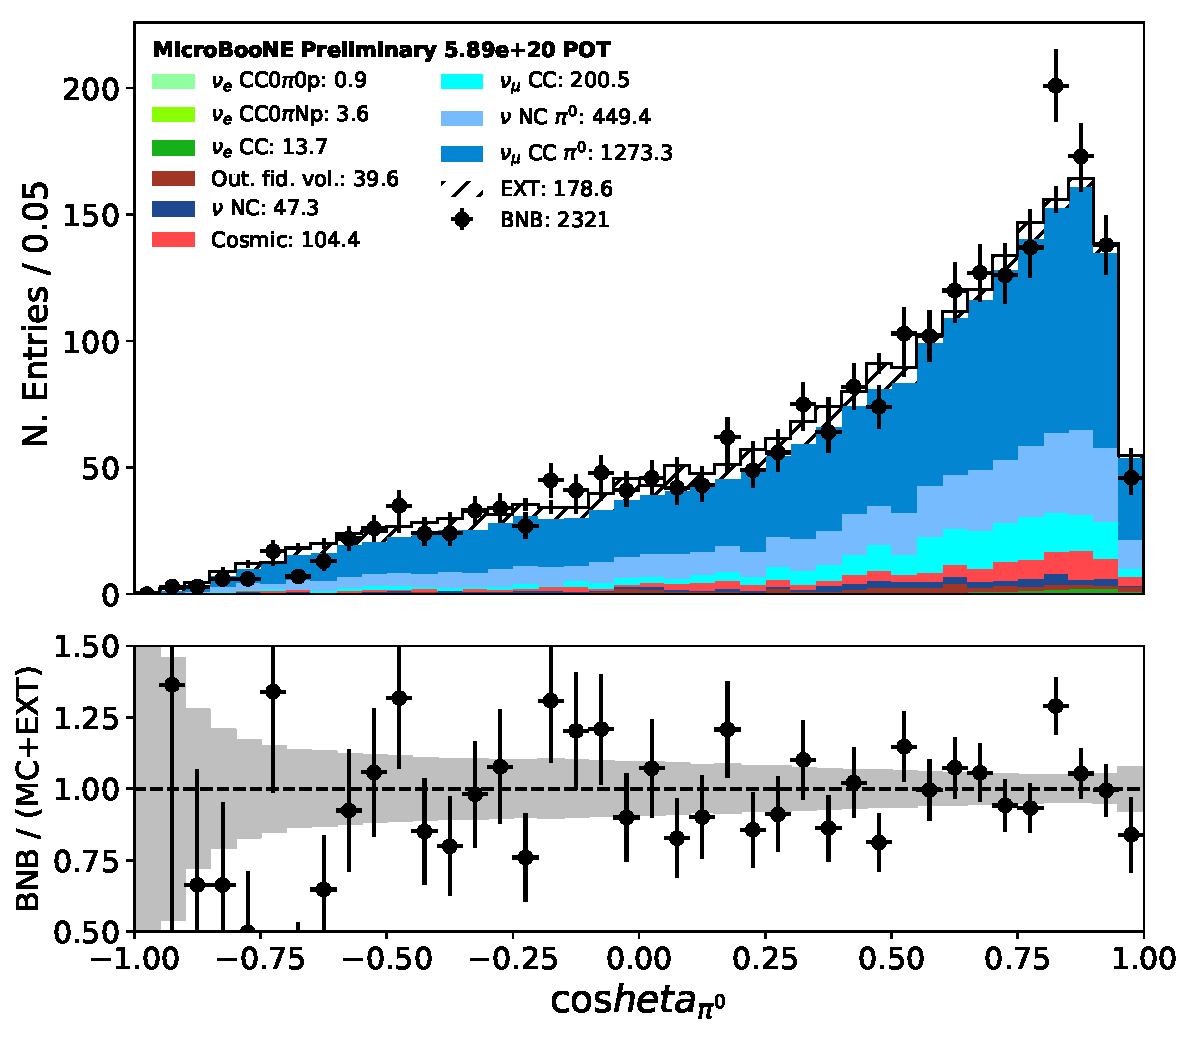
\includegraphics[width=1.00\textwidth]{pi0/kinematics/pi0momanglecos_03112020_ALL_scaled.pdf}
    \caption{}
    \end{subfigure}
    \begin{subfigure}[b]{0.3\textwidth}
    \centering
    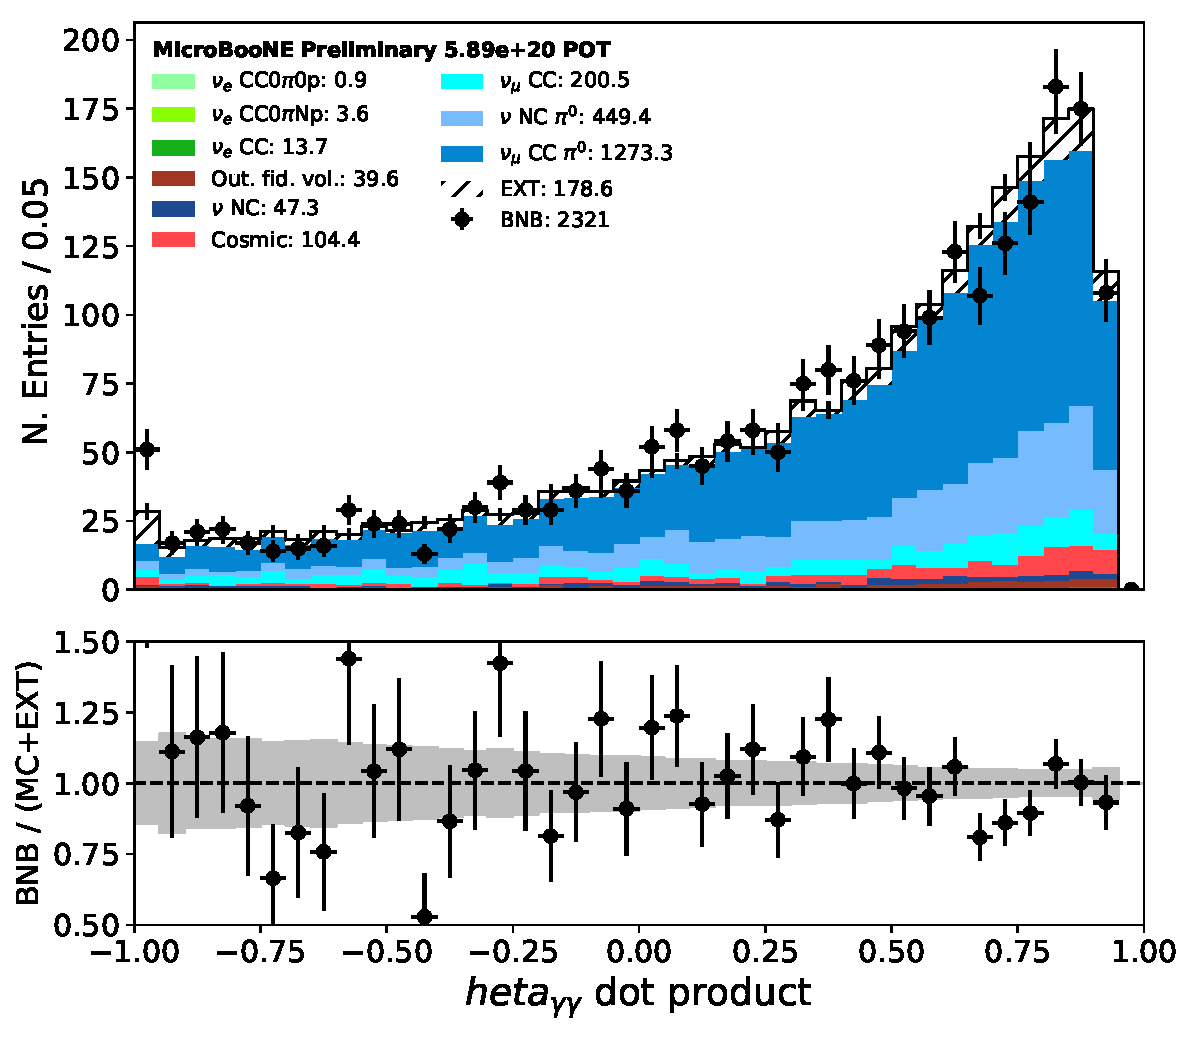
\includegraphics[width=1.00\textwidth]{pi0/kinematics/pi0_gammadot_03112020_ALL_scaled.pdf}
    \caption{}
    \end{subfigure}
\caption{Select $\pi^0$ kinematic distributions.}
\label{fig:pi0:kinematics:A}
\end{center}
\end{figure}

\begin{figure}[H] 
\begin{center}
    \begin{subfigure}[b]{0.3\textwidth}
    \centering
    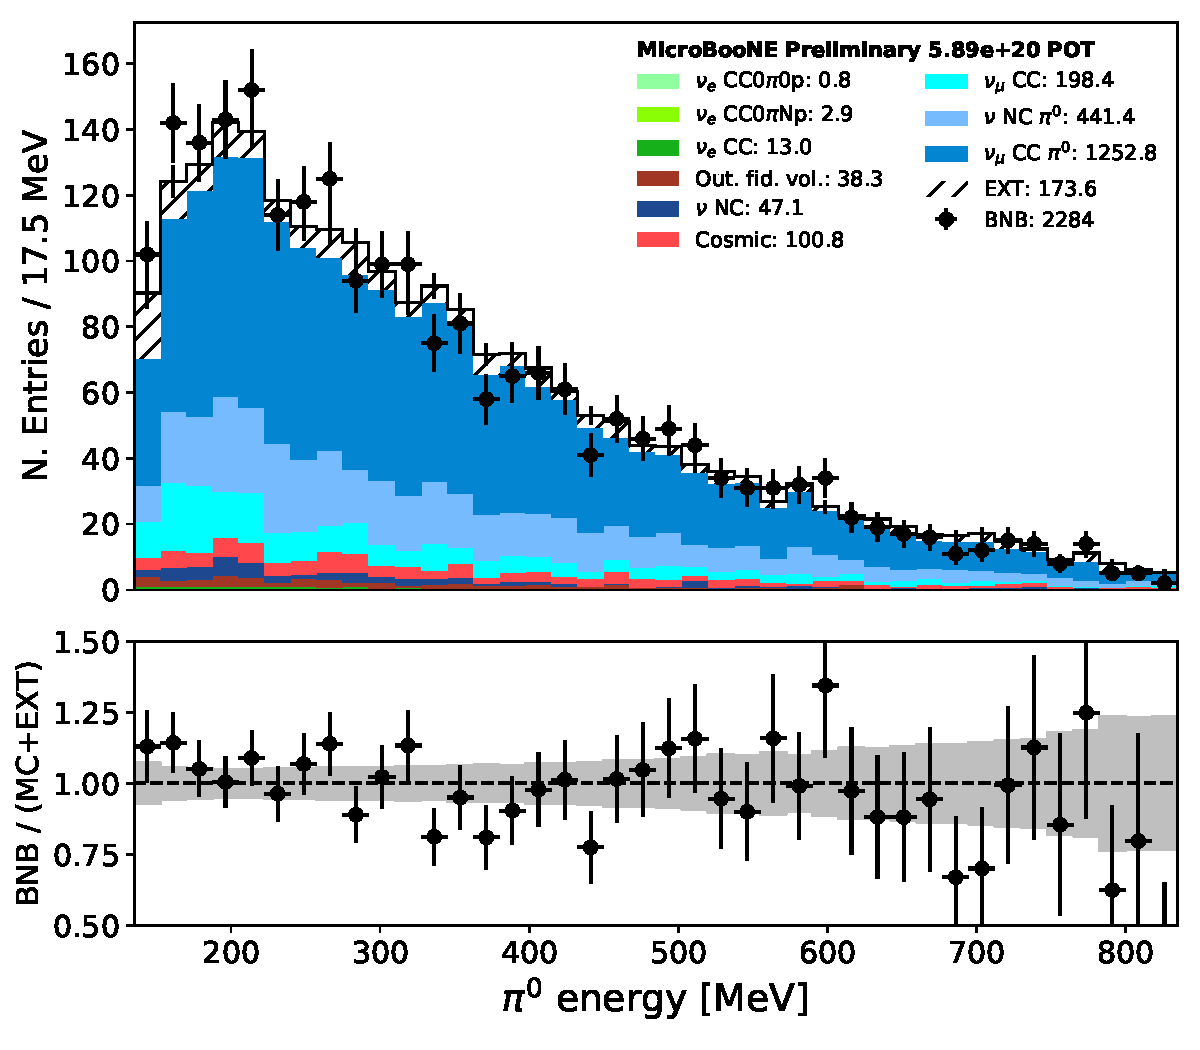
\includegraphics[width=1.00\textwidth]{pi0/kinematics/pi0energy_03112020_ALL_scaled.pdf}
    \caption{\label{fig:pi0:kinematics:pi0e} $\pi^0$ energy [GeV]}
    \end{subfigure}
    \begin{subfigure}[b]{0.3\textwidth}
    \centering
    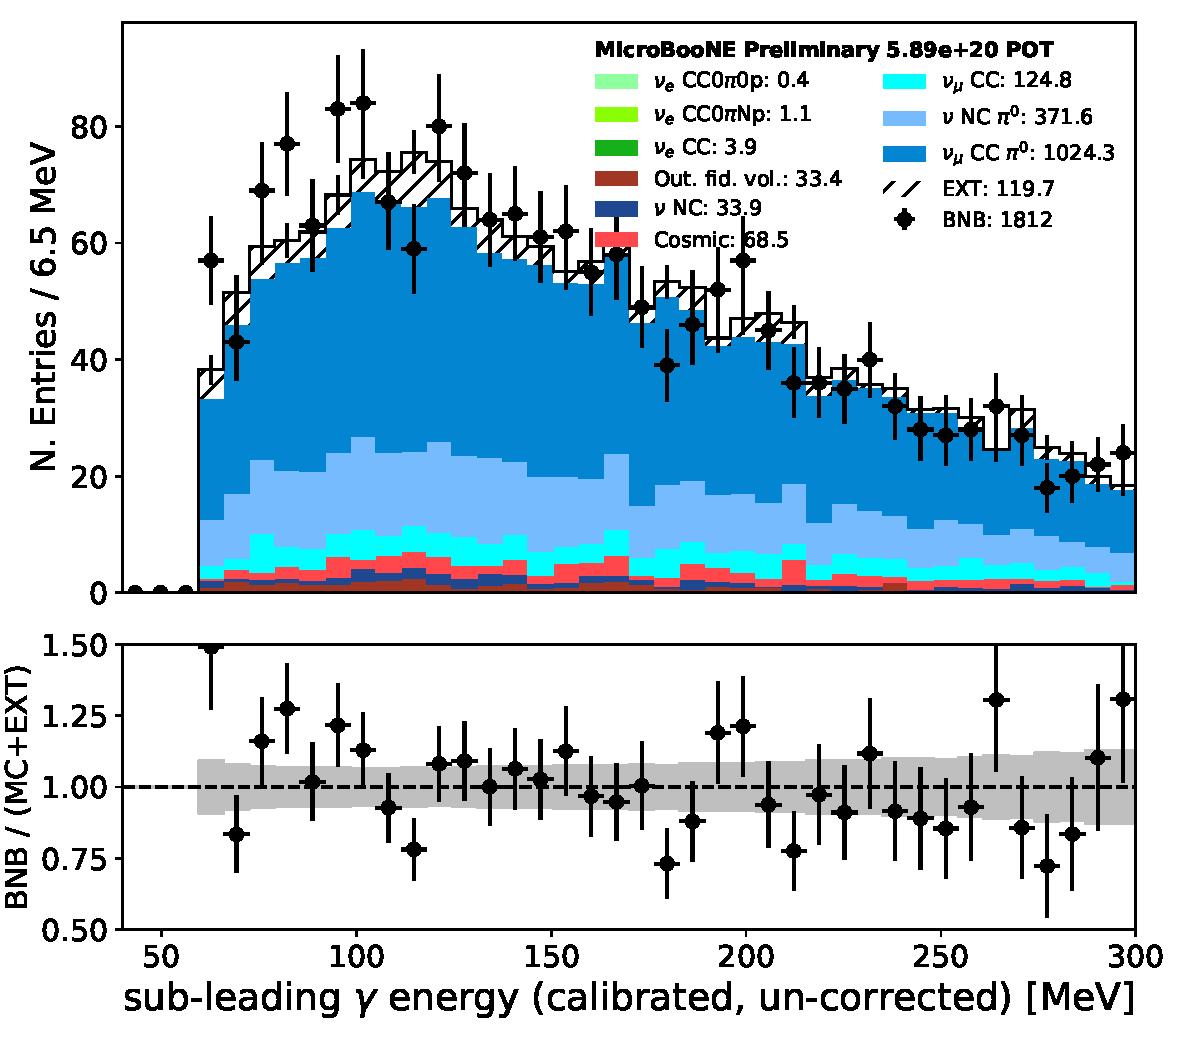
\includegraphics[width=1.00\textwidth]{pi0/kinematics/pi0_energy1_Y_03112020_ALL_scaled.pdf}
    \caption{}
    \end{subfigure}
    \begin{subfigure}[b]{0.3\textwidth}
    \centering
    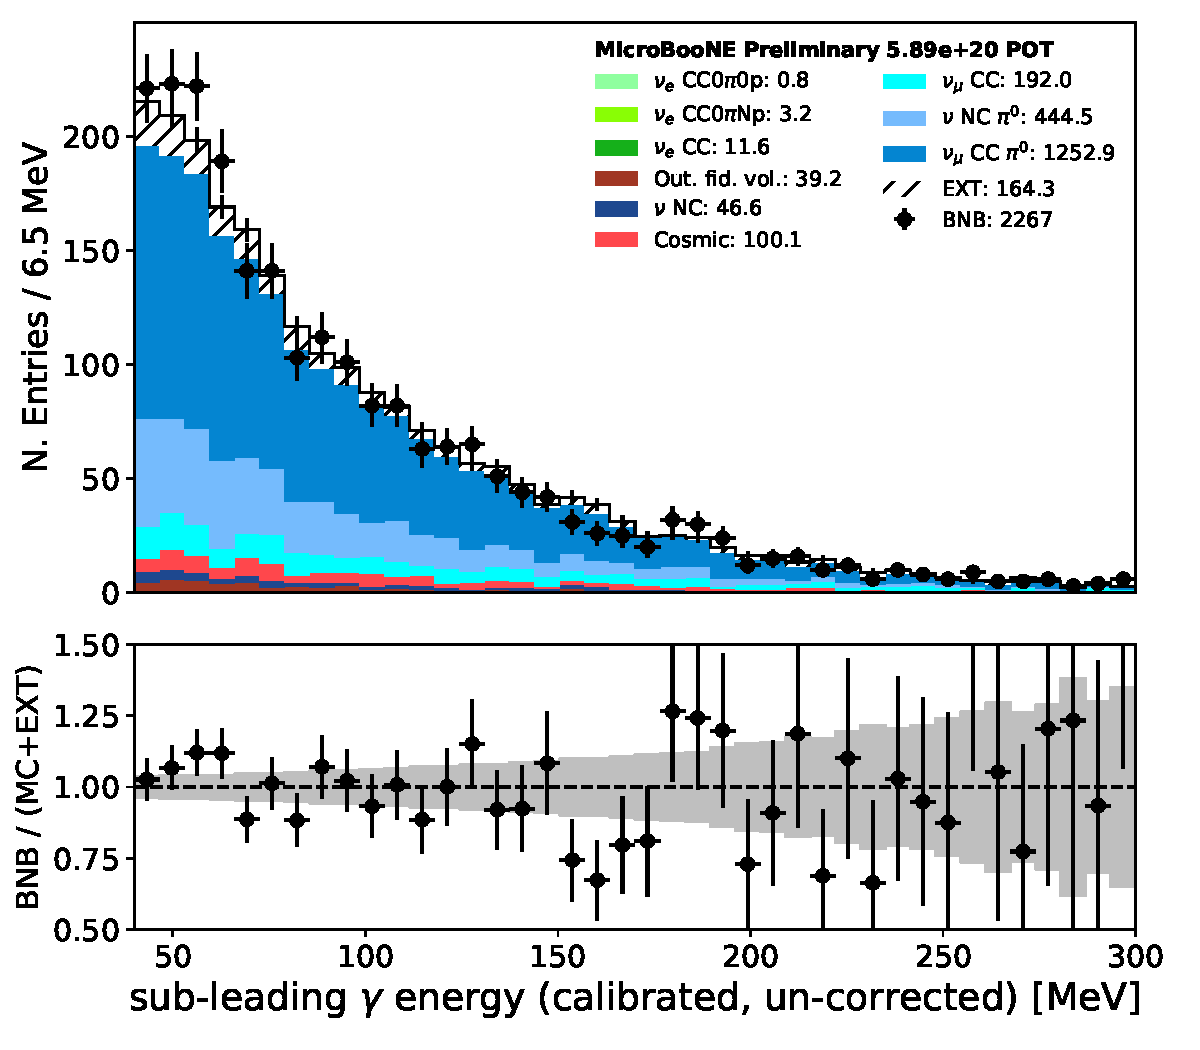
\includegraphics[width=1.00\textwidth]{pi0/kinematics/pi0_energy2_Y_03112020_ALL_scaled.pdf}
    \caption{}
    \end{subfigure}
\caption{Select $\pi^0$ kinematic distributions.}
\label{fig:pi0:kinematics:B}
\end{center}
\end{figure}

\begin{figure}[H] 
\begin{center}
    \begin{subfigure}[b]{0.3\textwidth}
    \centering
    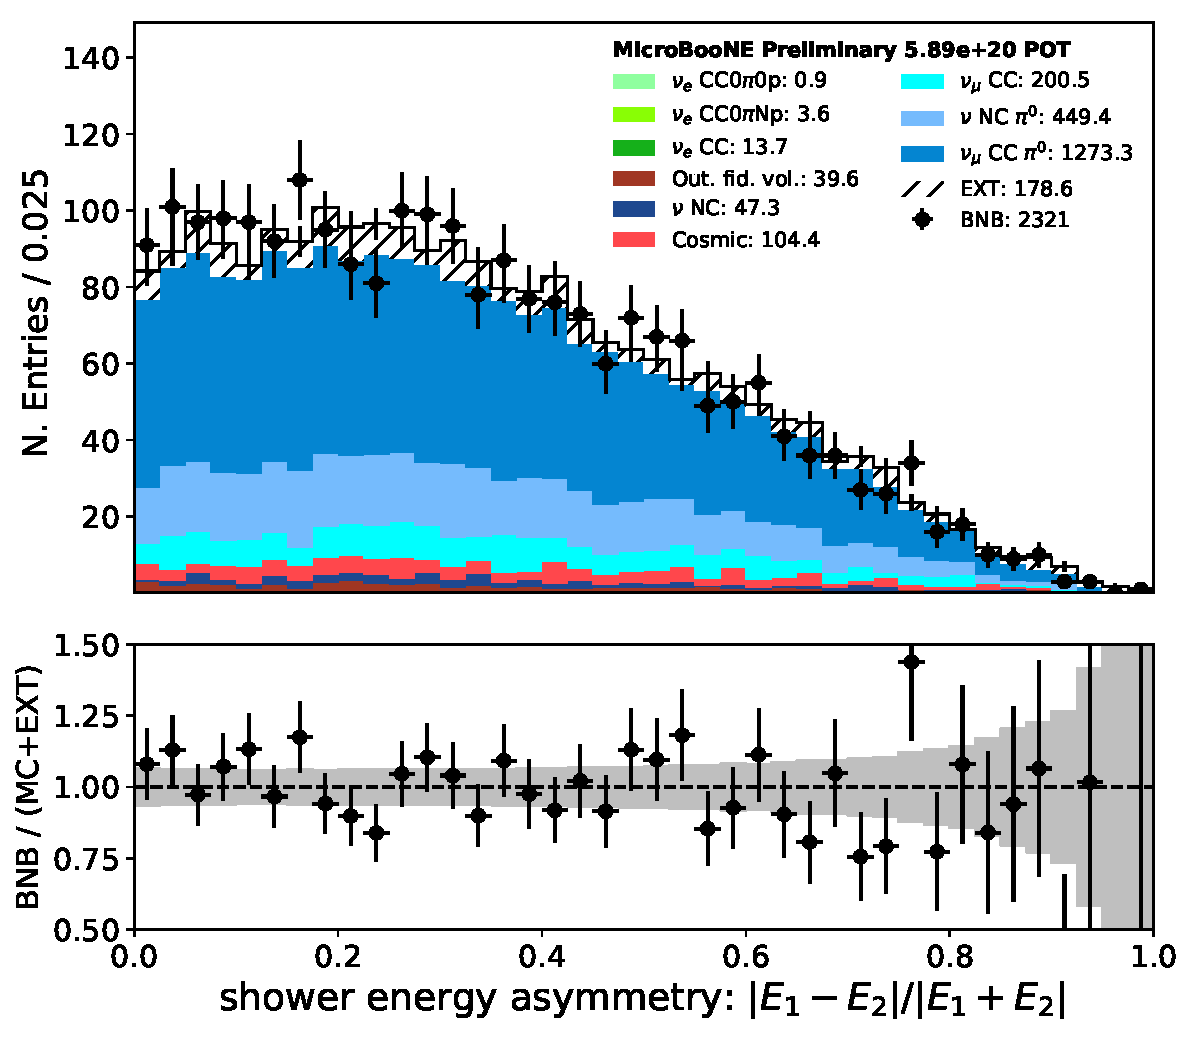
\includegraphics[width=1.00\textwidth]{pi0/kinematics/asymm_03112020_ALL_scaled.pdf}
    \caption{}
    \end{subfigure}
    \begin{subfigure}[b]{0.3\textwidth}
    \centering
    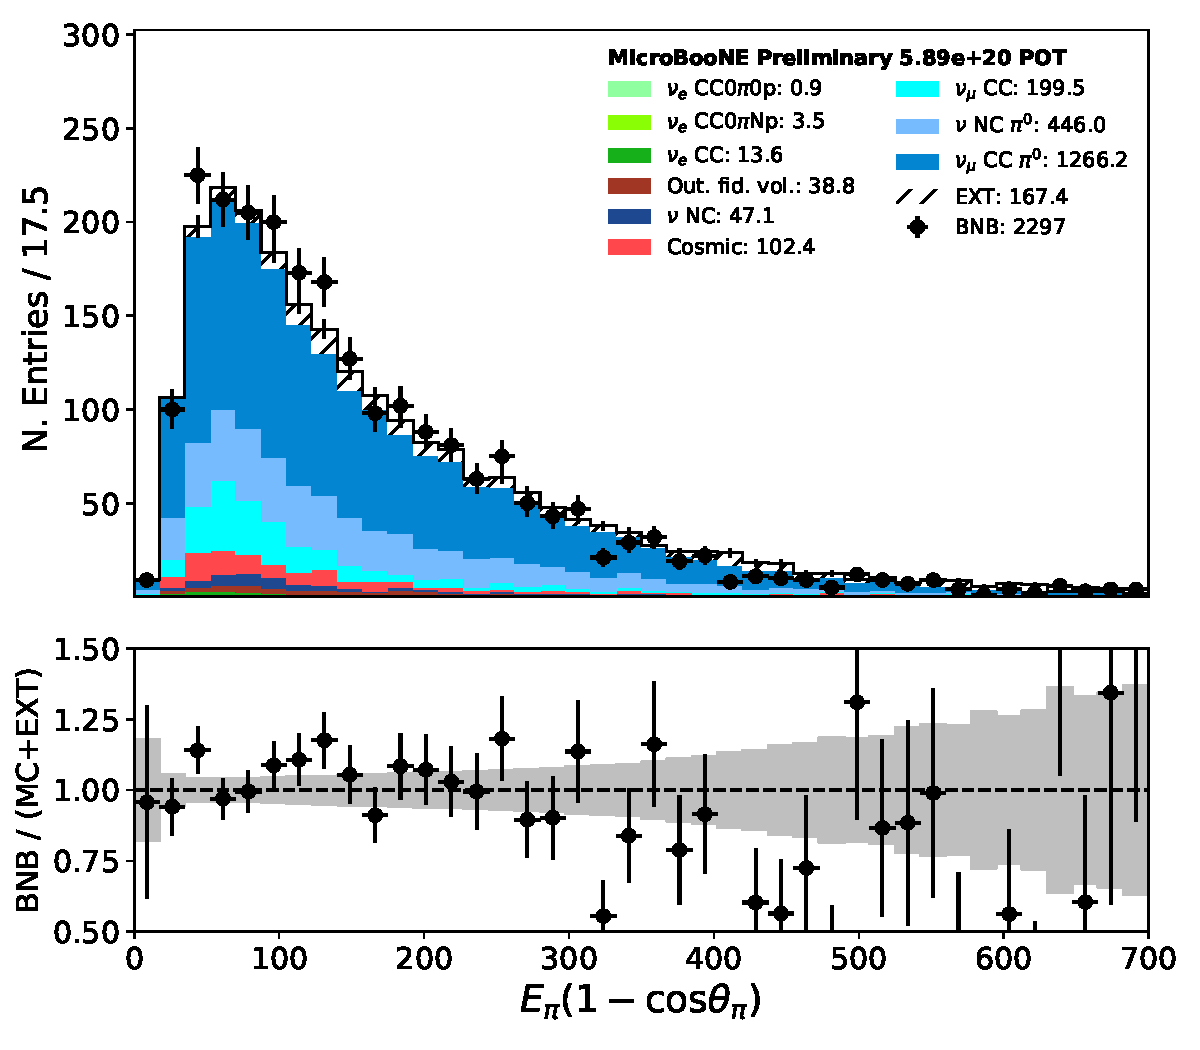
\includegraphics[width=1.00\textwidth]{pi0/kinematics/epicospi_03112020_ALL_scaled.pdf}
    \caption{}
    \end{subfigure}
\caption{Select $\pi^0$ kinematic distributions.}
\label{fig:pi0:kinematics:C}
\end{center}
\end{figure}


\subsection{$\pi^0$ calorimetric variables}
\label{app:pi0:calorimetry}

\begin{figure}[H] 
\begin{center}
    \begin{subfigure}[b]{0.3\textwidth}
    \centering
    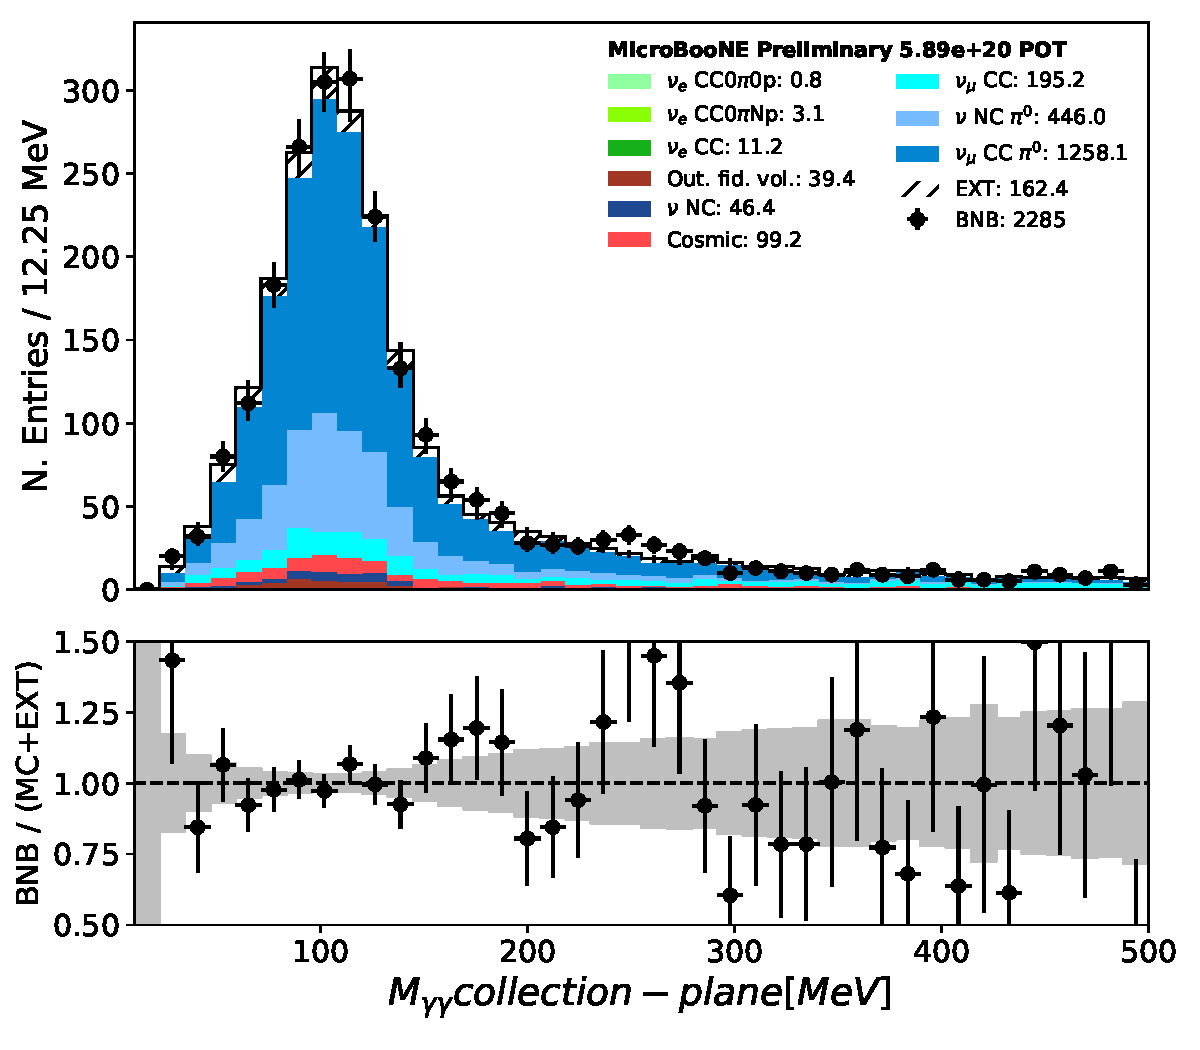
\includegraphics[width=1.00\textwidth]{pi0/calorimetry/pi0_mass_Y_03112020_ALL_scaled.pdf}
    \caption{}
    \end{subfigure}
    \begin{subfigure}[b]{0.3\textwidth}
    \centering
    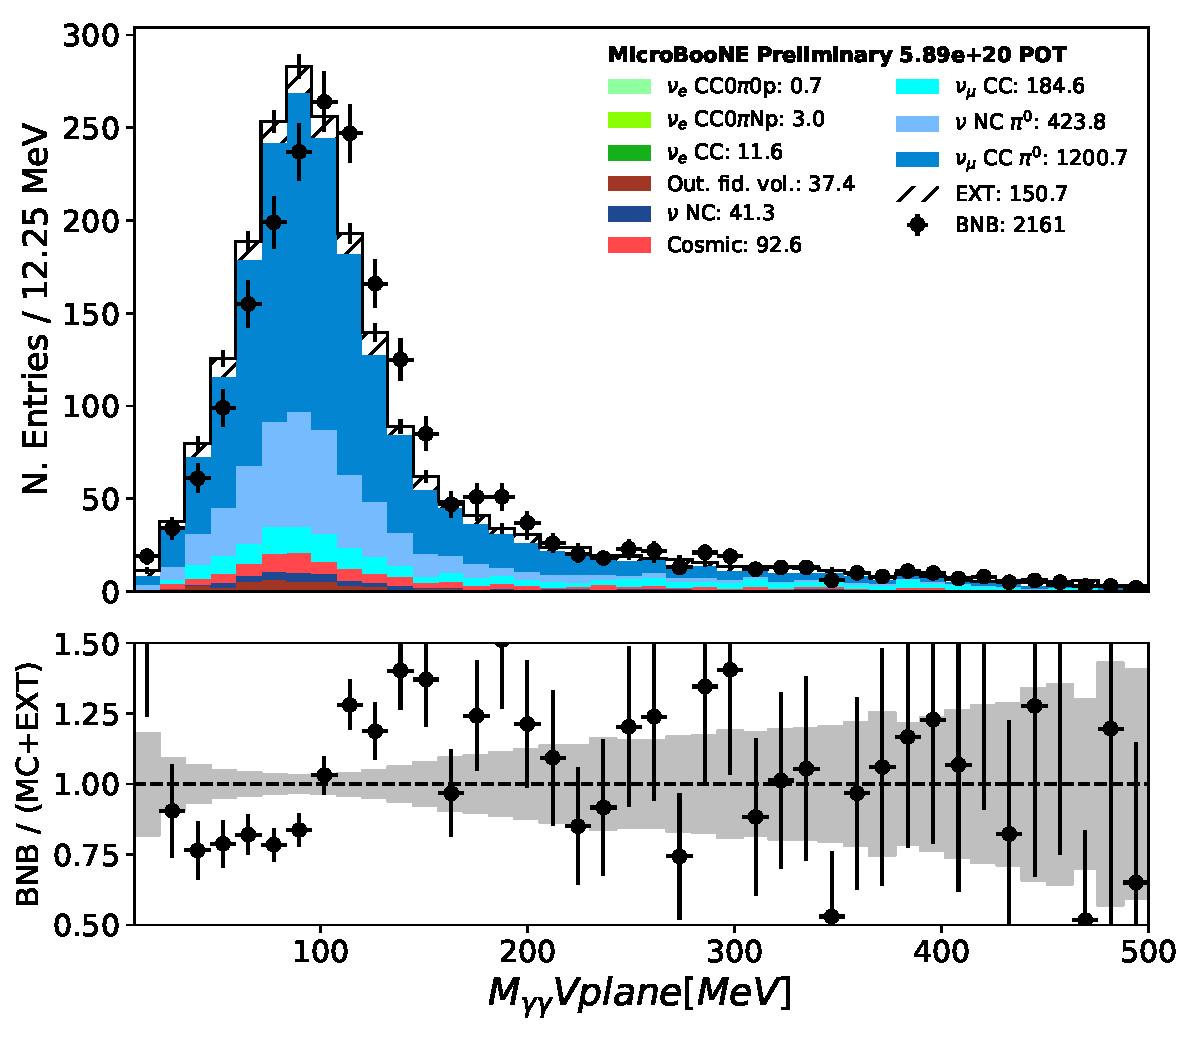
\includegraphics[width=1.00\textwidth]{pi0/calorimetry/pi0_mass_V_03112020_ALL_scaled.pdf}
    \caption{}
    \end{subfigure}
    \begin{subfigure}[b]{0.3\textwidth}
    \centering
    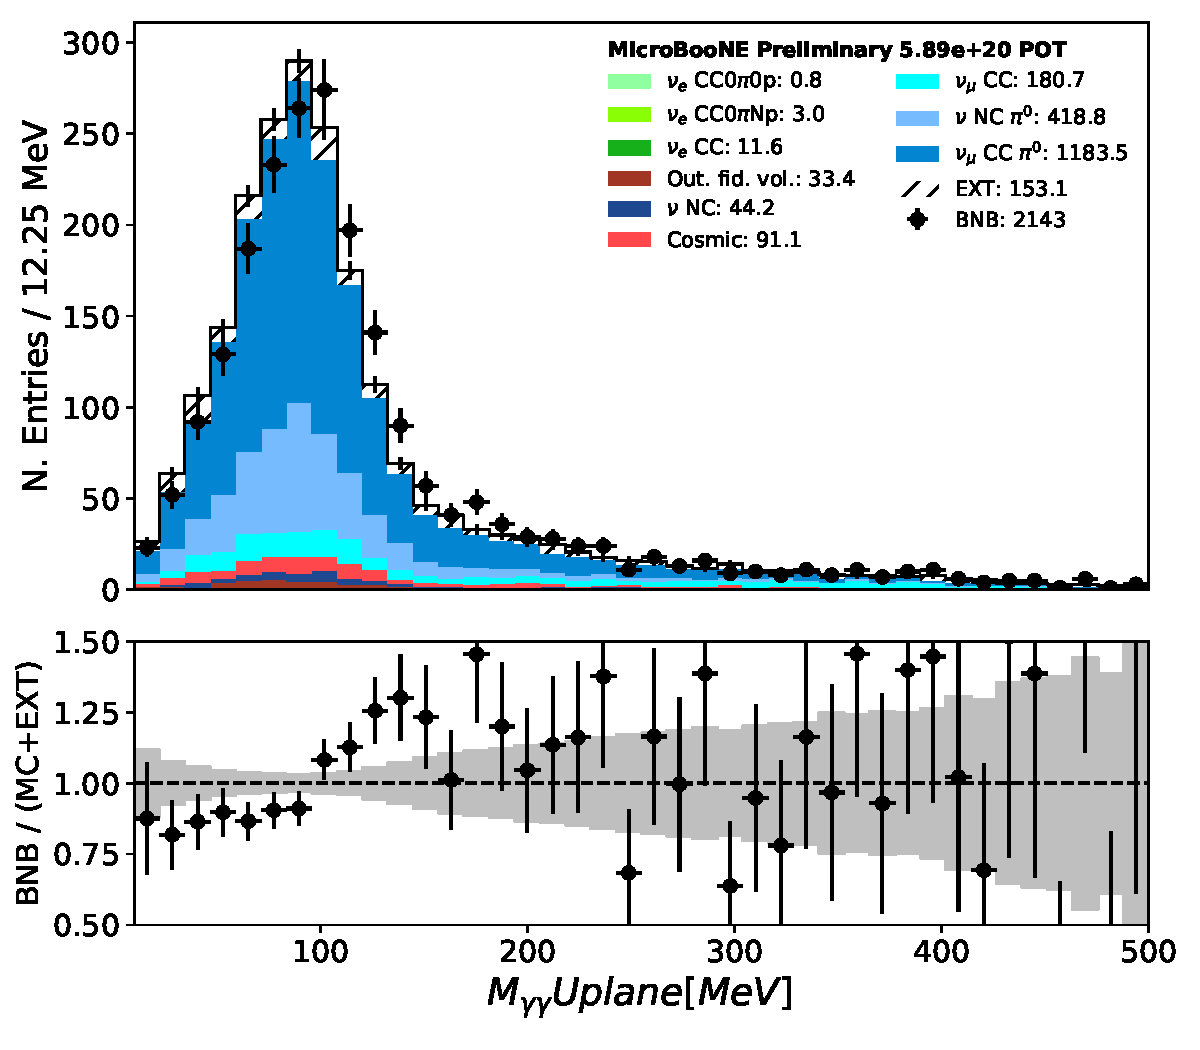
\includegraphics[width=1.00\textwidth]{pi0/calorimetry/pi0_mass_U_03112020_ALL_scaled.pdf}
    \caption{}
    \end{subfigure}
\caption{$M_{\gamma\gamma}$ for Y/V/U planes. Calibrated but not bias-corrected.}
\label{fig:pi0:calorimetry:mass}
\end{center}
\end{figure}

\begin{figure}[H] 
\begin{center}
    \begin{subfigure}[b]{0.3\textwidth}
    \centering
    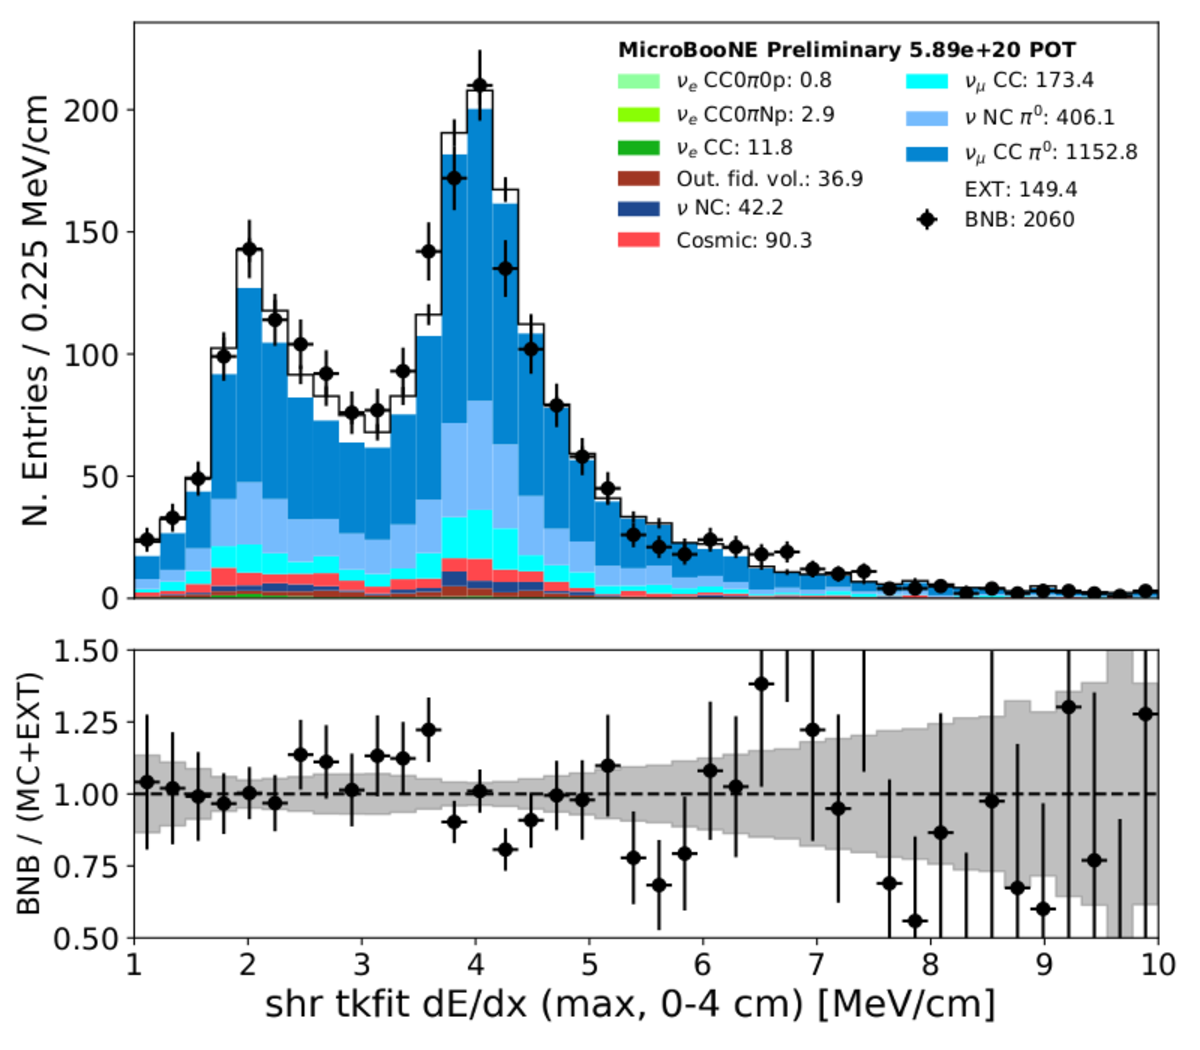
\includegraphics[width=1.00\textwidth]{pi0/calorimetry/shr_tkfit_dedx_max_03112020_ALL_scaled.pdf}
    \caption{all showers}
    \end{subfigure}
    \begin{subfigure}[b]{0.3\textwidth}
    \centering
    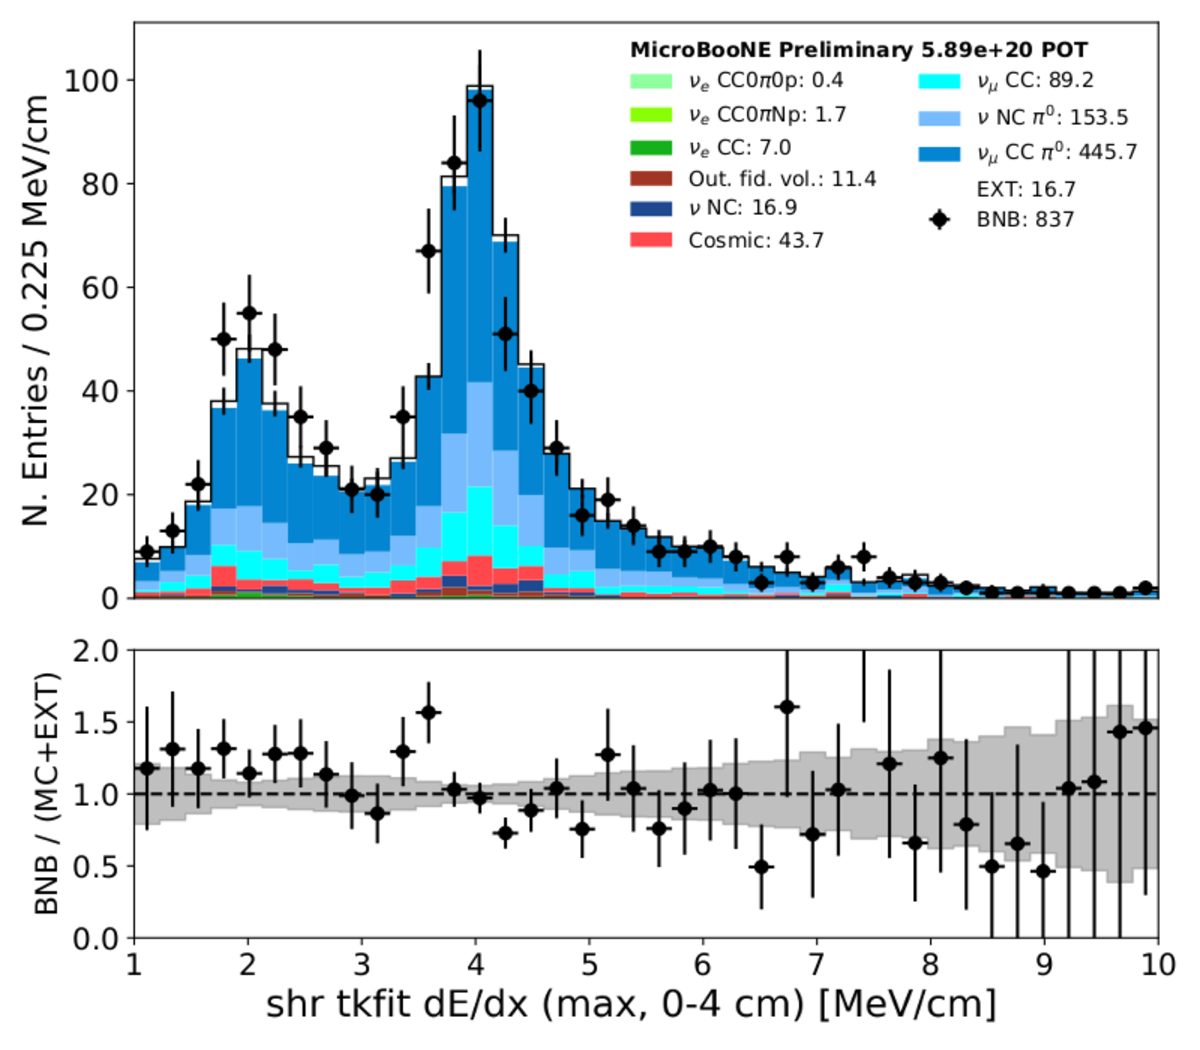
\includegraphics[width=1.00\textwidth]{pi0/calorimetry/shr_tkfit_dedx_max_03112020_ALL_scaled_pz075.pdf}
    \caption{shower $P_z > 0.75$}
    \end{subfigure}
\caption{Reconstructed dE/dx on ``best'' plane.}
\label{fig:pi0:calorimetry:dedxbest}
\end{center}
\end{figure}

\begin{figure}[H] 
\begin{center}
    \begin{subfigure}[b]{0.3\textwidth}
    \centering
    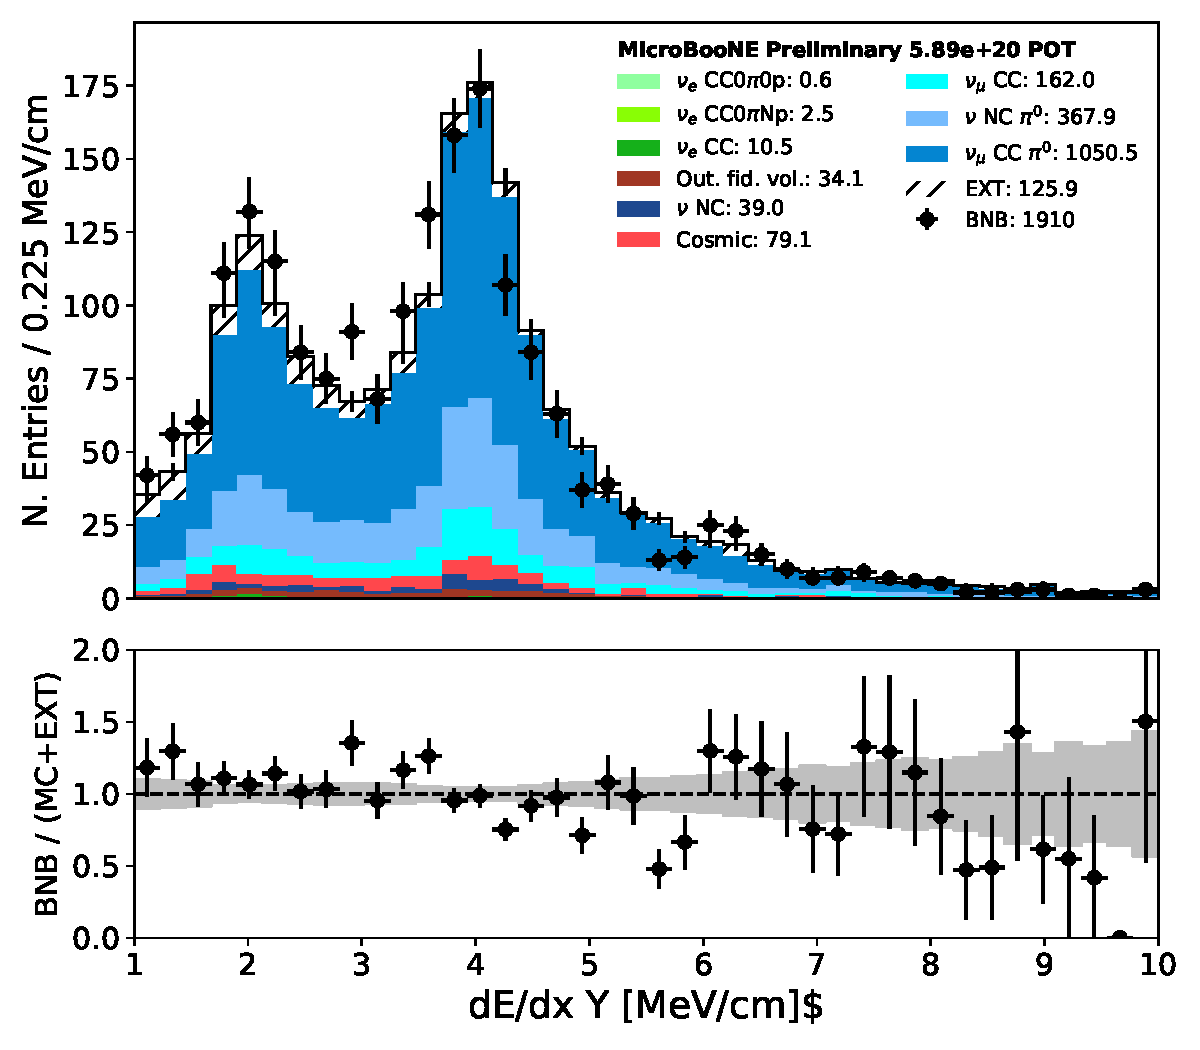
\includegraphics[width=1.00\textwidth]{pi0/calorimetry/shr_tkfit_dedx_Y_03112020_ALL_scaled.pdf}
    \caption{}
    \end{subfigure}
    \begin{subfigure}[b]{0.3\textwidth}
    \centering
    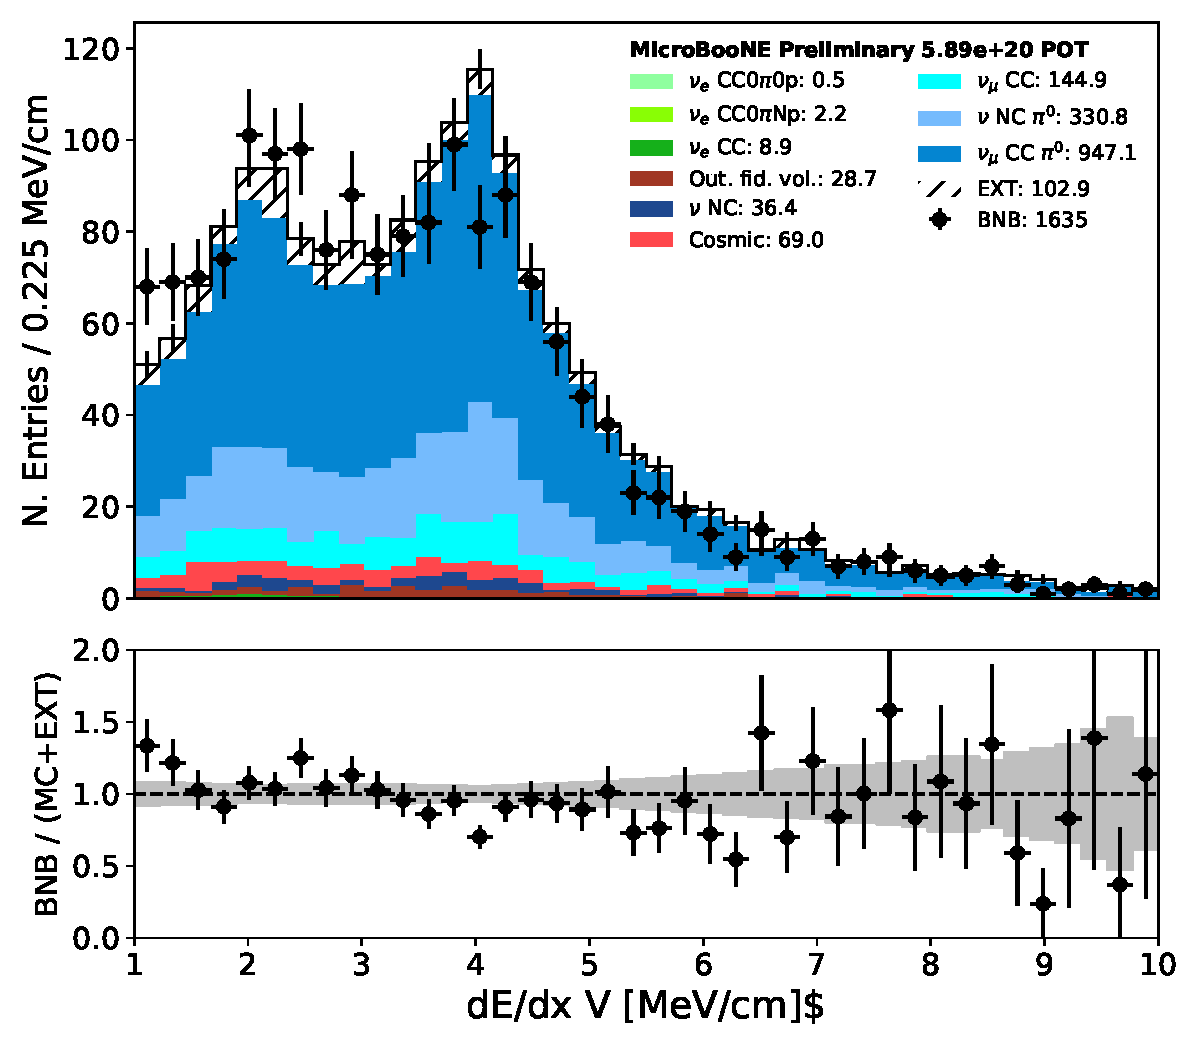
\includegraphics[width=1.00\textwidth]{pi0/calorimetry/shr_tkfit_dedx_V_03112020_ALL_scaled.pdf}
    \caption{}
    \end{subfigure}
    \begin{subfigure}[b]{0.3\textwidth}
    \centering
    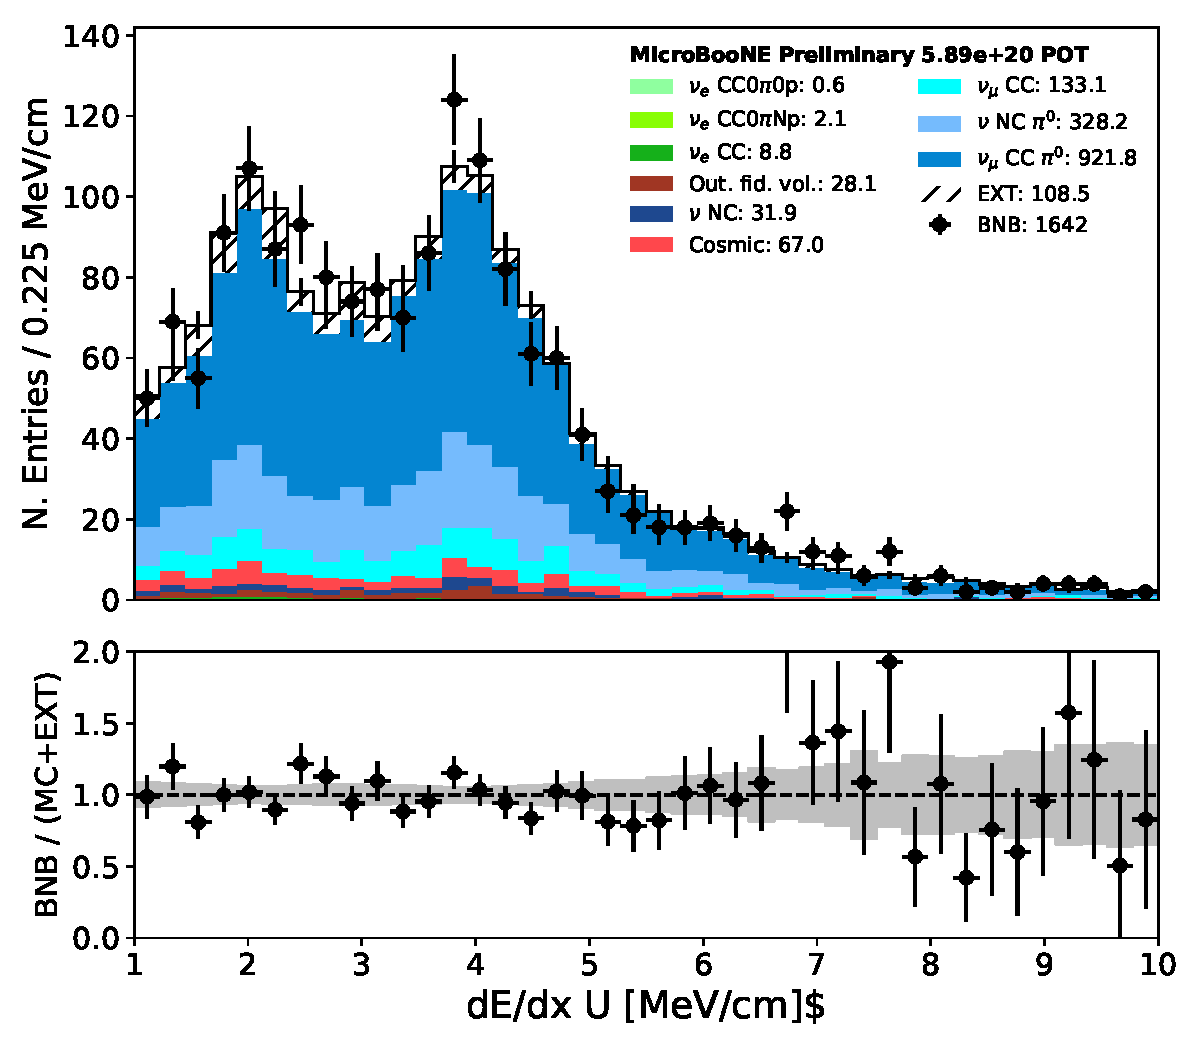
\includegraphics[width=1.00\textwidth]{pi0/calorimetry/shr_tkfit_dedx_U_03112020_ALL_scaled.pdf}
    \caption{}
    \end{subfigure}
\caption{dE/dx for Y/V/U planes}
\label{fig:pi0:calorimetry:dedx}
\end{center}
\end{figure}

\begin{figure}[H] 
\begin{center}
    \begin{subfigure}[b]{0.3\textwidth}
    \centering
    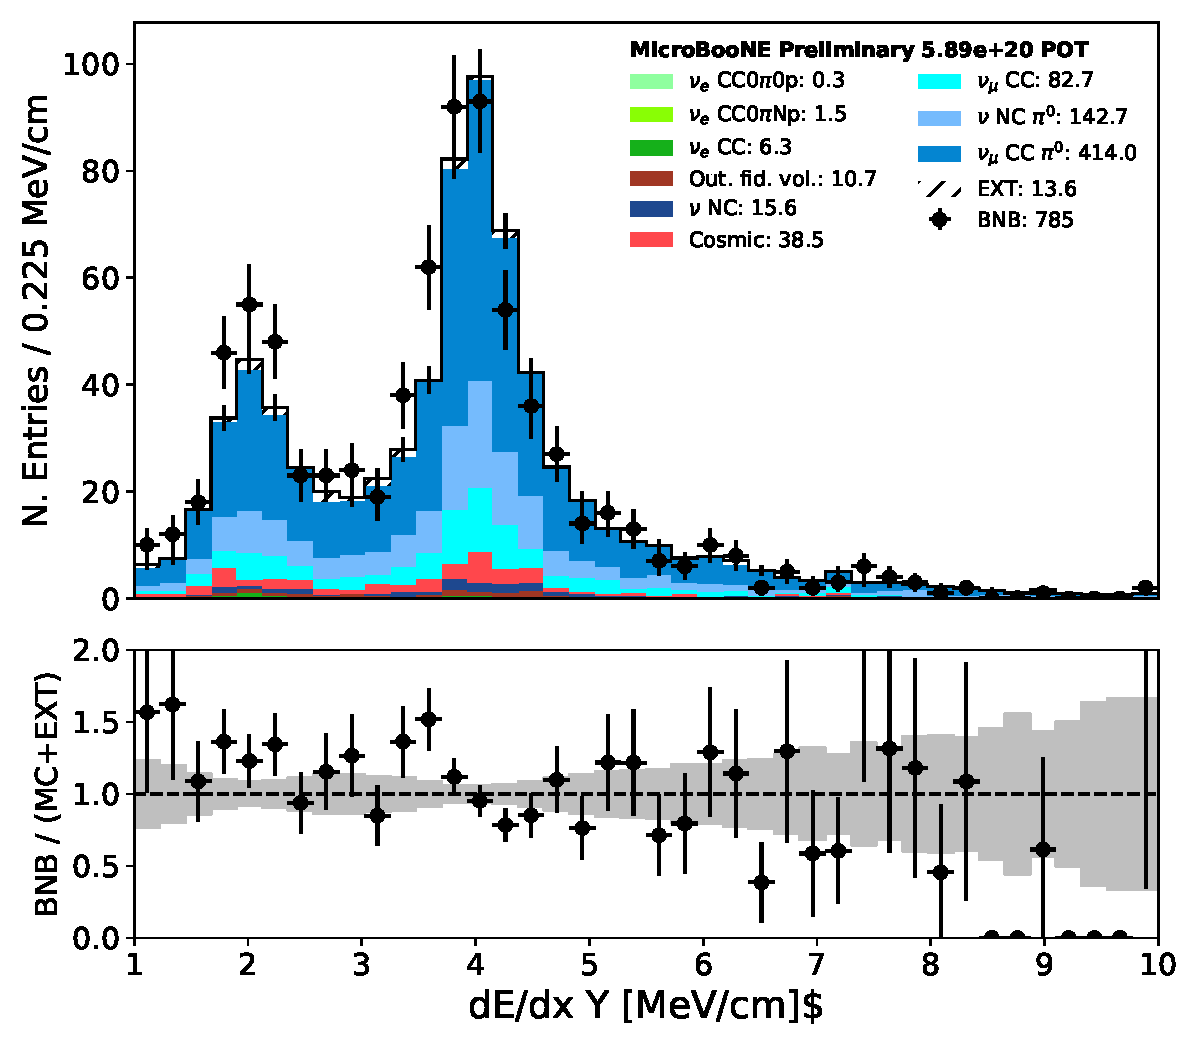
\includegraphics[width=1.00\textwidth]{pi0/calorimetry/shr_tkfit_dedx_Y_03112020_ALL_scaled_pz075.pdf}
    \caption{}
    \end{subfigure}
    \begin{subfigure}[b]{0.3\textwidth}
    \centering
    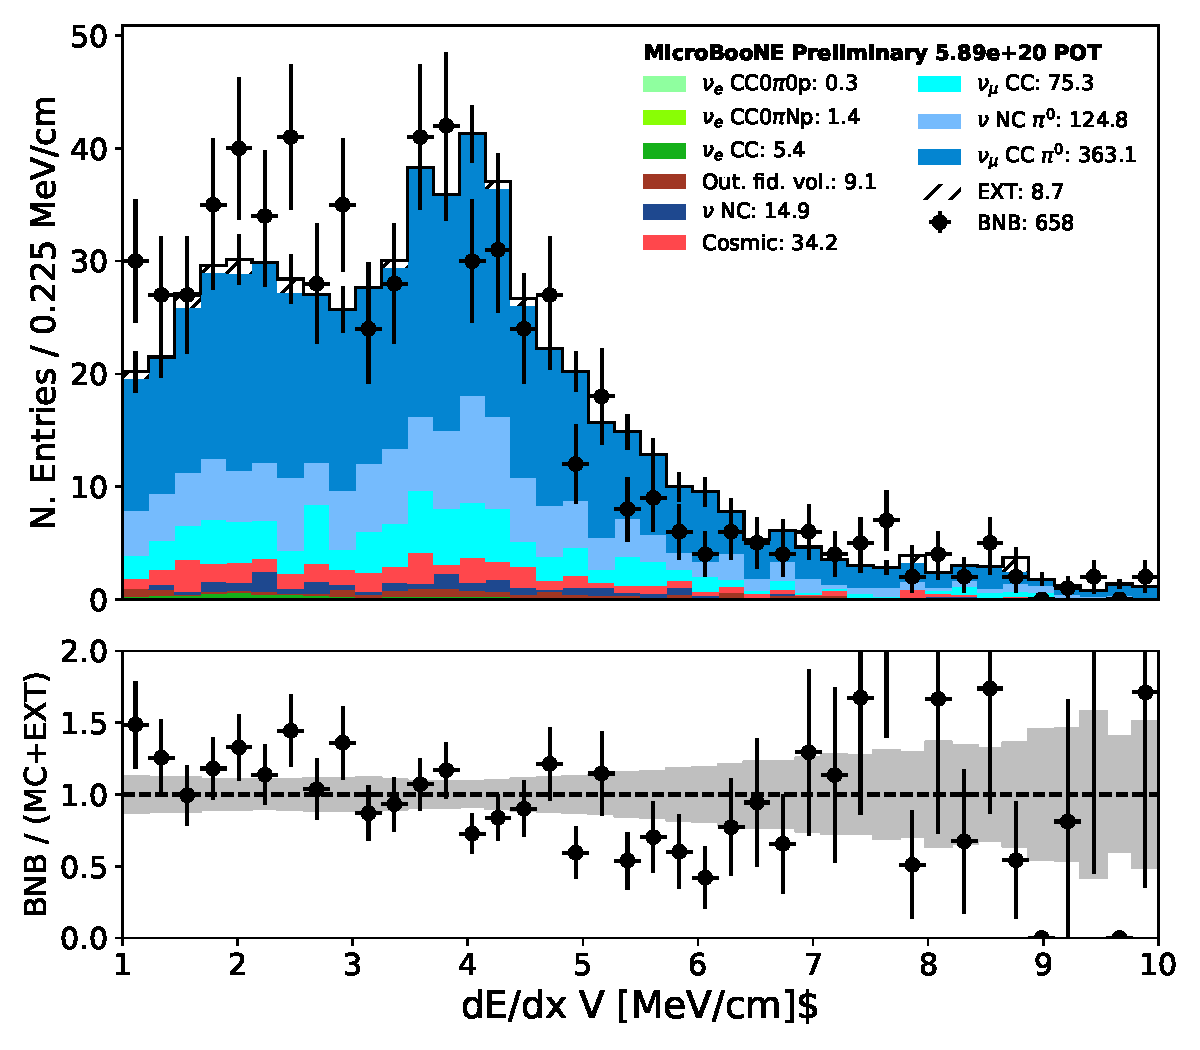
\includegraphics[width=1.00\textwidth]{pi0/calorimetry/shr_tkfit_dedx_V_03112020_ALL_scaled_pz075.pdf}
    \caption{}
    \end{subfigure}
    \begin{subfigure}[b]{0.3\textwidth}
    \centering
    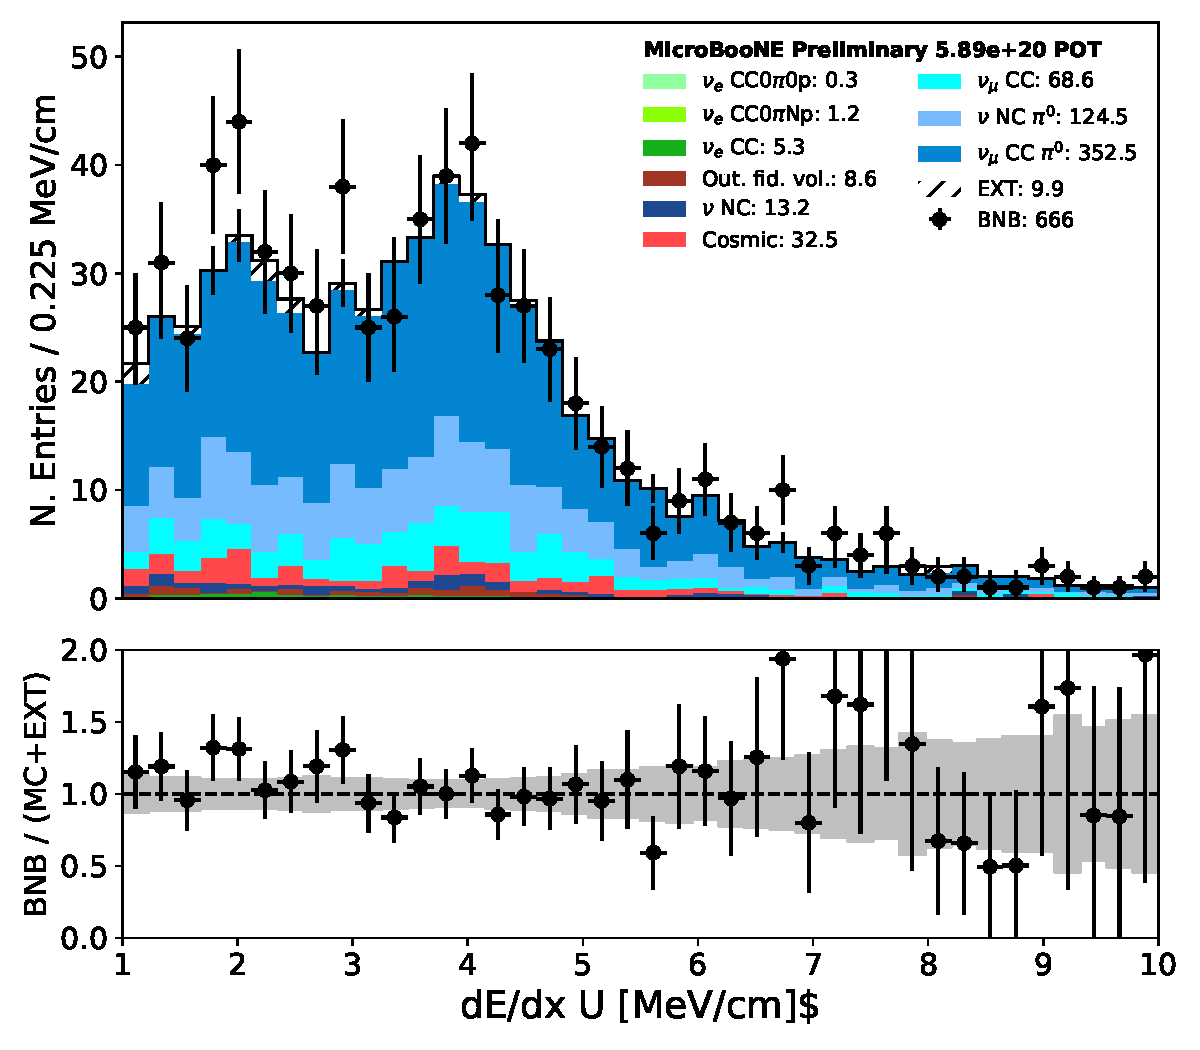
\includegraphics[width=1.00\textwidth]{pi0/calorimetry/shr_tkfit_dedx_U_03112020_ALL_scaled_pz075.pdf}
    \caption{}
    \end{subfigure}
\caption{dE/dx for Y/V/U planes for showers with $P_z > 0.75$.}
\label{fig:pi0:calorimetry:dedxpz}
\end{center}
\end{figure}

\begin{figure}[H] 
\begin{center}
    \begin{subfigure}[b]{0.3\textwidth}
    \centering
    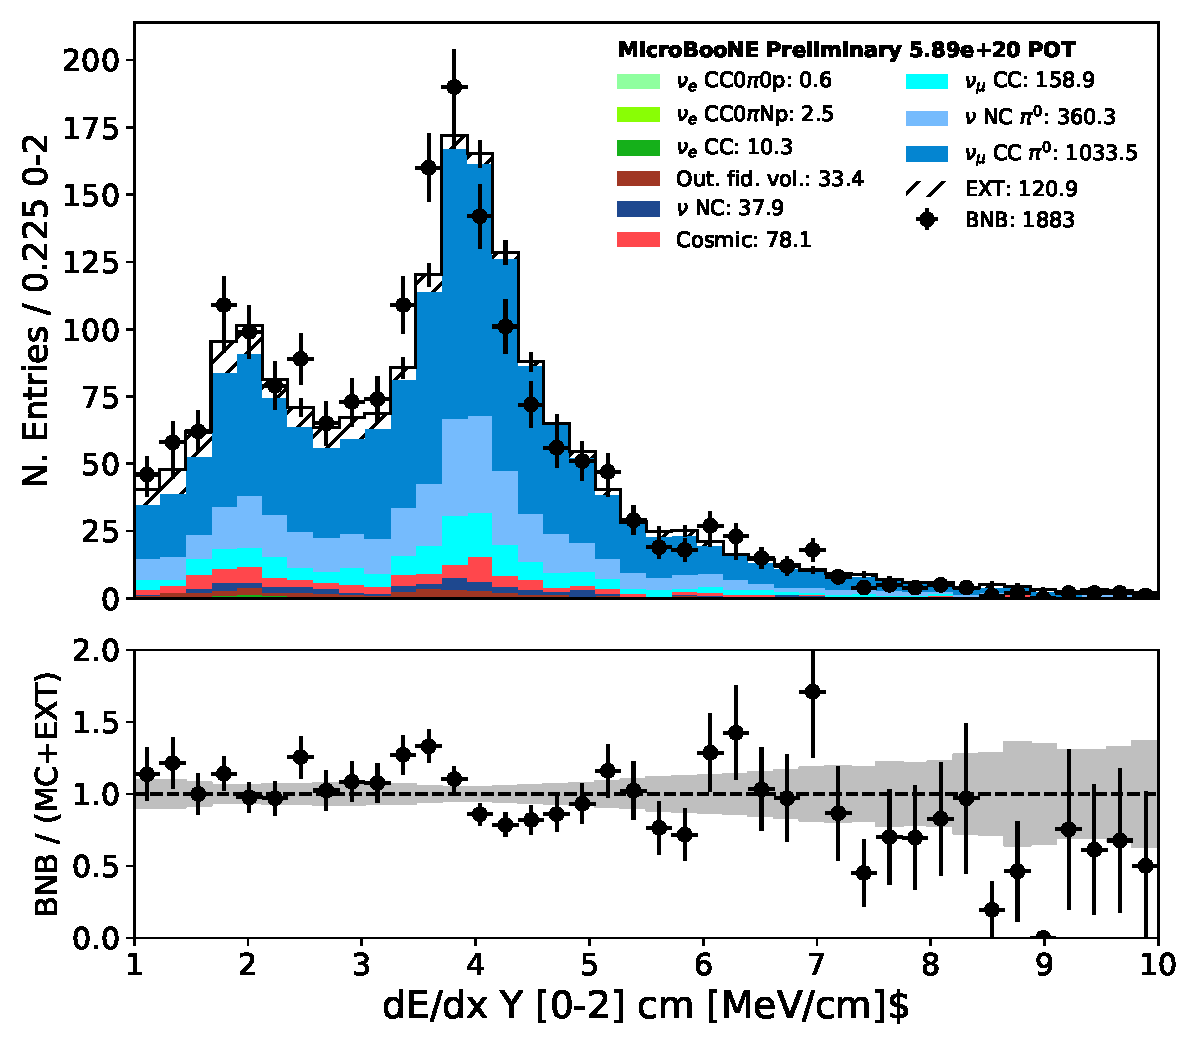
\includegraphics[width=1.00\textwidth]{pi0/calorimetry/shr_tkfit_2cm_dedx_Y_03112020_ALL_scaled.pdf}
    \caption{}
    \end{subfigure}
    \begin{subfigure}[b]{0.3\textwidth}
    \centering
    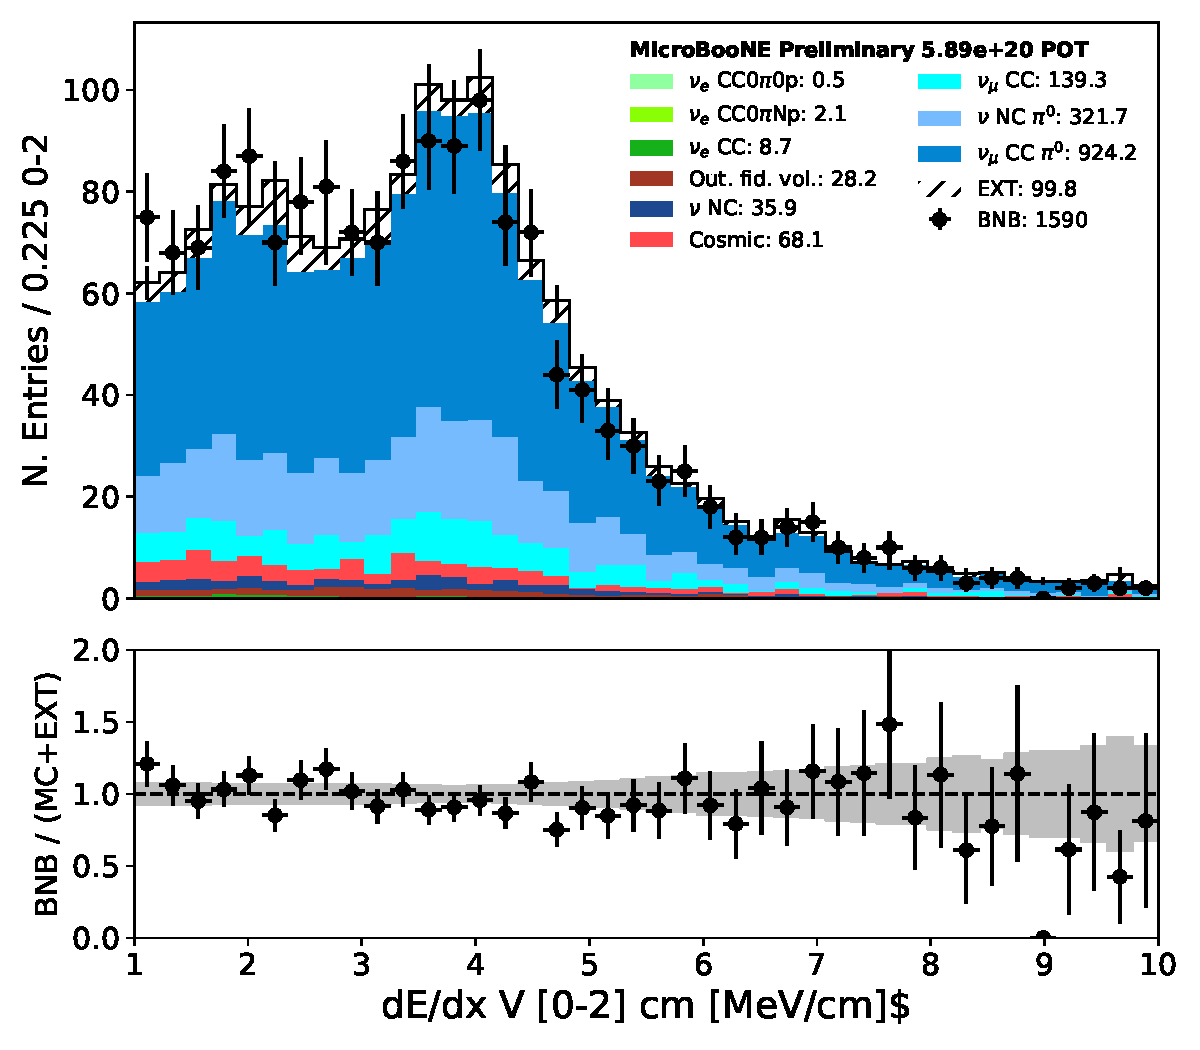
\includegraphics[width=1.00\textwidth]{pi0/calorimetry/shr_tkfit_2cm_dedx_V_03112020_ALL_scaled.pdf}
    \caption{}
    \end{subfigure}
    \begin{subfigure}[b]{0.3\textwidth}
    \centering
    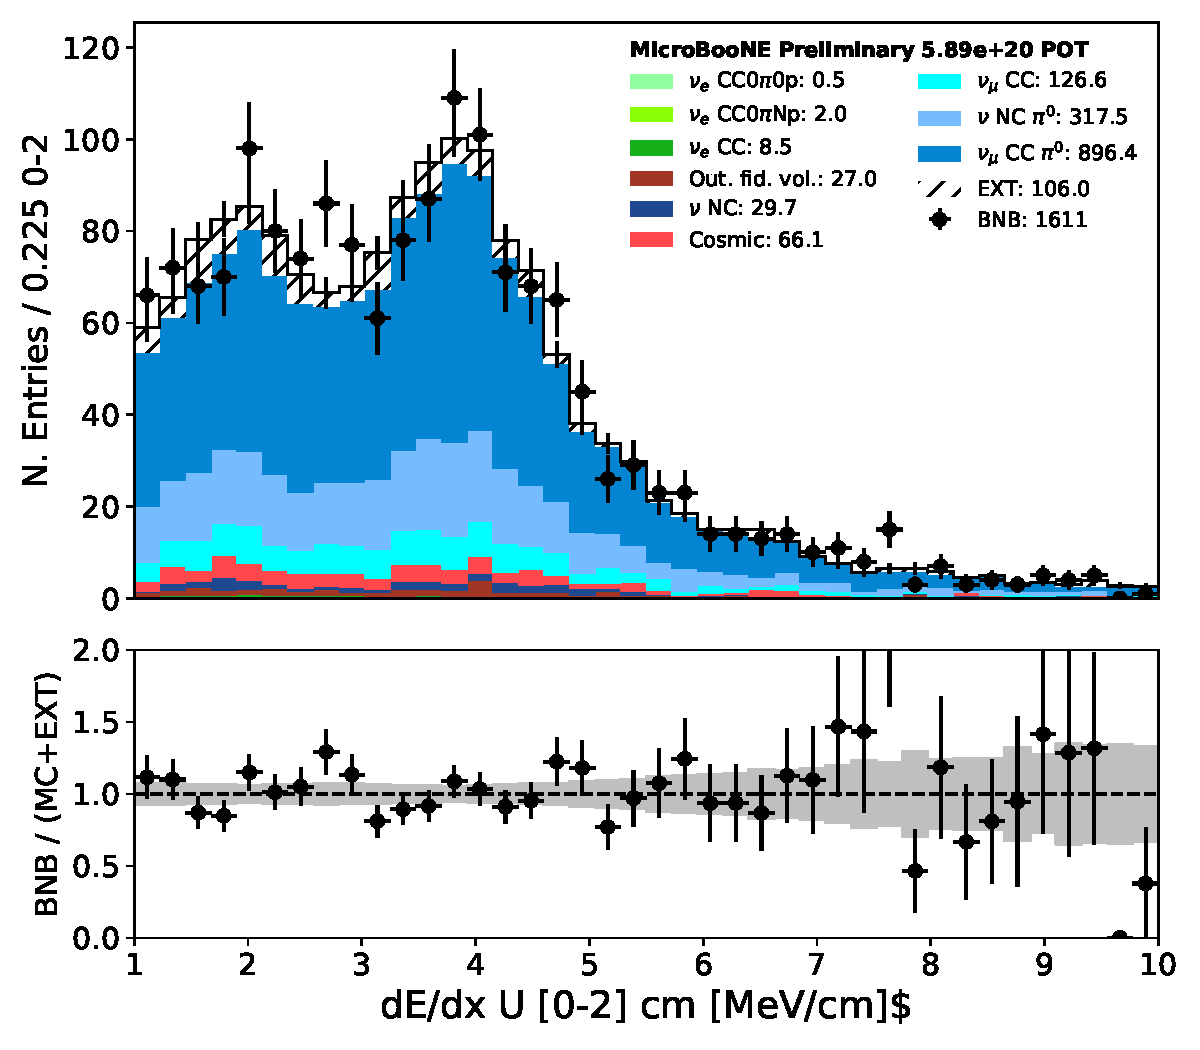
\includegraphics[width=1.00\textwidth]{pi0/calorimetry/shr_tkfit_2cm_dedx_U_03112020_ALL_scaled.pdf}
    \caption{}
    \end{subfigure}
\caption{dE/dx for Y/V/U planes computed over first 2 cm of shower trunk.}
\label{fig:pi0:calorimetry:dedx2cm}
\end{center}
\end{figure}

\begin{figure}[H] 
\begin{center}
    \begin{subfigure}[b]{0.3\textwidth}
    \centering
    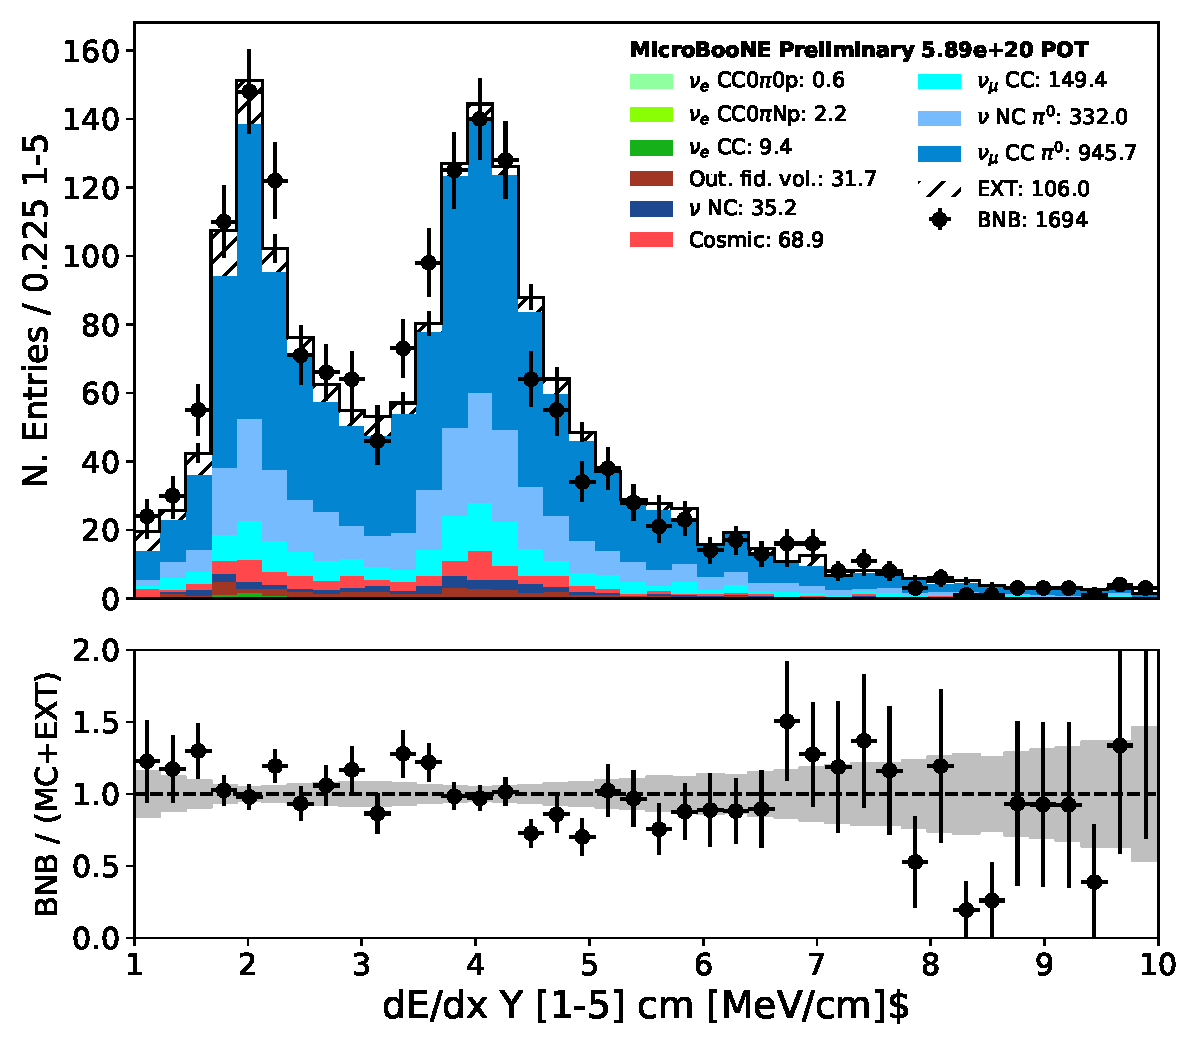
\includegraphics[width=1.00\textwidth]{pi0/calorimetry/shr_tkfit_gap10_dedx_Y_03112020_ALL_scaled.pdf}
    \caption{}
    \end{subfigure}
    \begin{subfigure}[b]{0.3\textwidth}
    \centering
    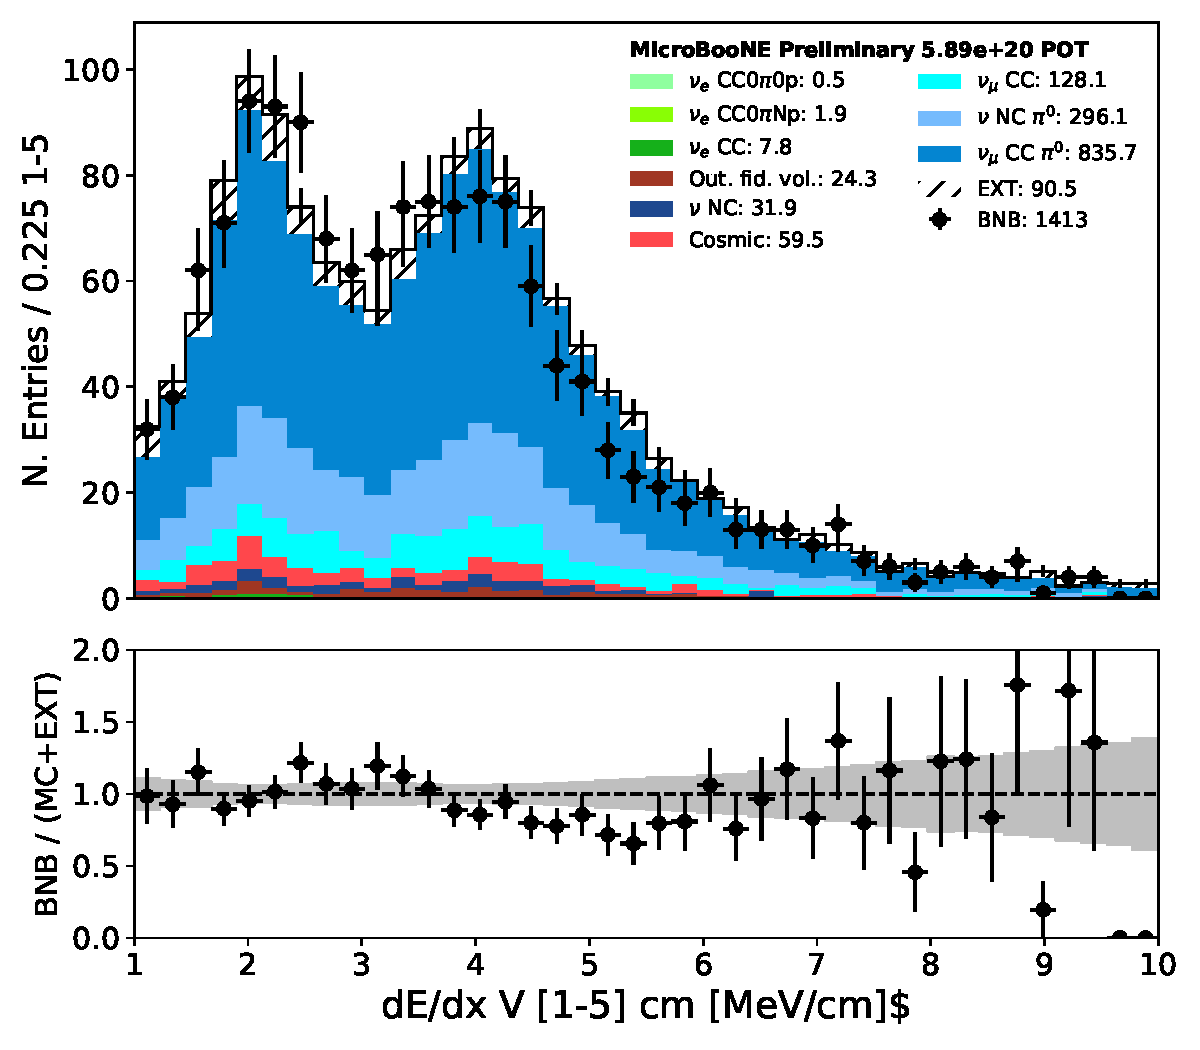
\includegraphics[width=1.00\textwidth]{pi0/calorimetry/shr_tkfit_gap10_dedx_V_03112020_ALL_scaled.pdf}
    \caption{}
    \end{subfigure}
    \begin{subfigure}[b]{0.3\textwidth}
    \centering
    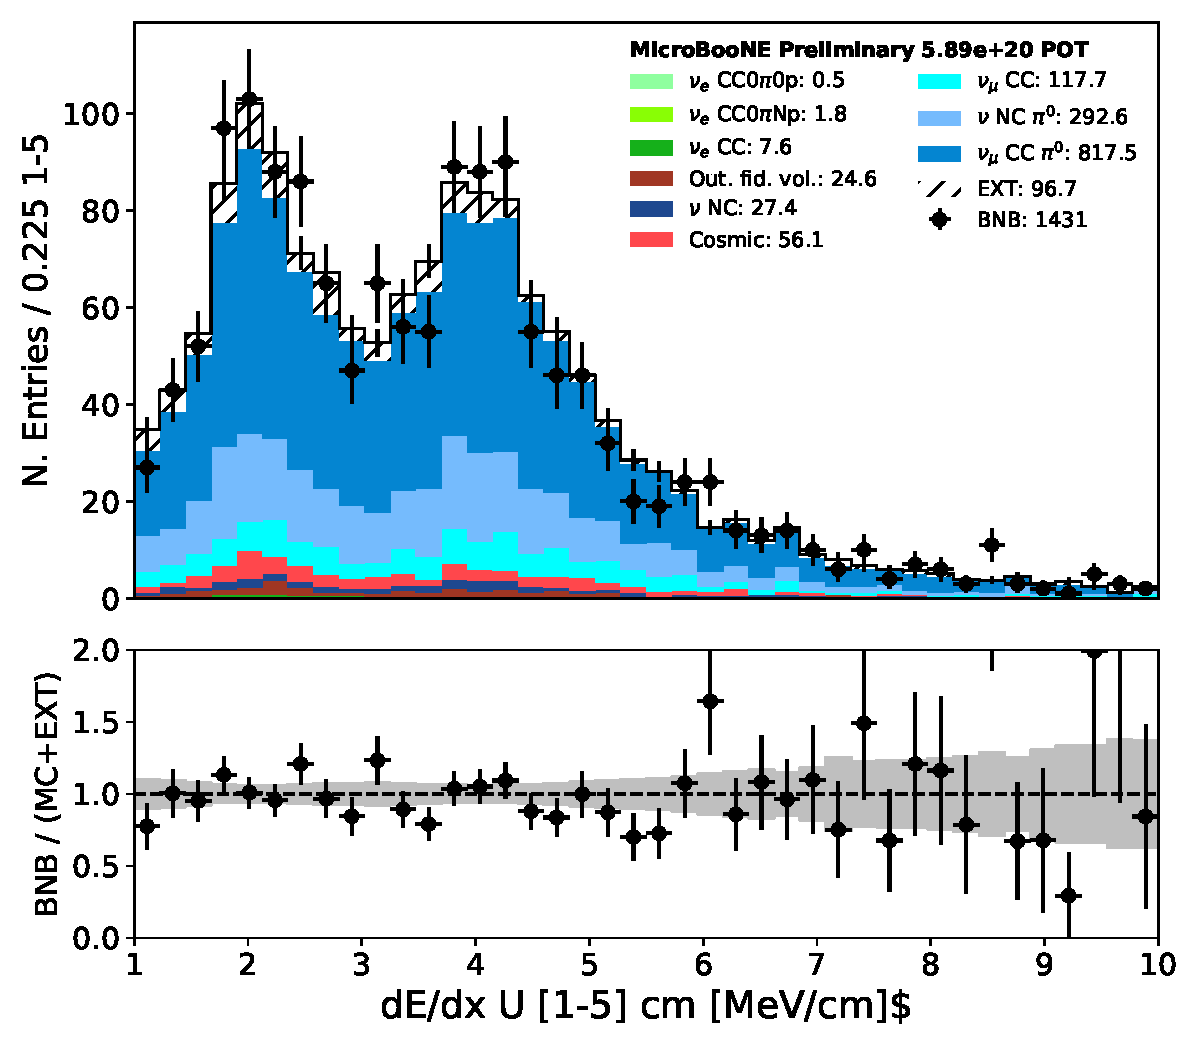
\includegraphics[width=1.00\textwidth]{pi0/calorimetry/shr_tkfit_gap10_dedx_U_03112020_ALL_scaled.pdf}
    \caption{}
    \end{subfigure}
\caption{dE/dx for Y/V/U planes computed over range [1-5] cm of shower trunk.}
\label{fig:pi0:calorimetry:dedxgap10}
\end{center}
\end{figure}

\subsection{$\nu_e$ input variable distributions in $\pi^0$ sideband}
\label{app:pi0:nueselection}

\begin{figure}[H] 
\begin{center}
    \begin{subfigure}[b]{0.3\textwidth}
    \centering
    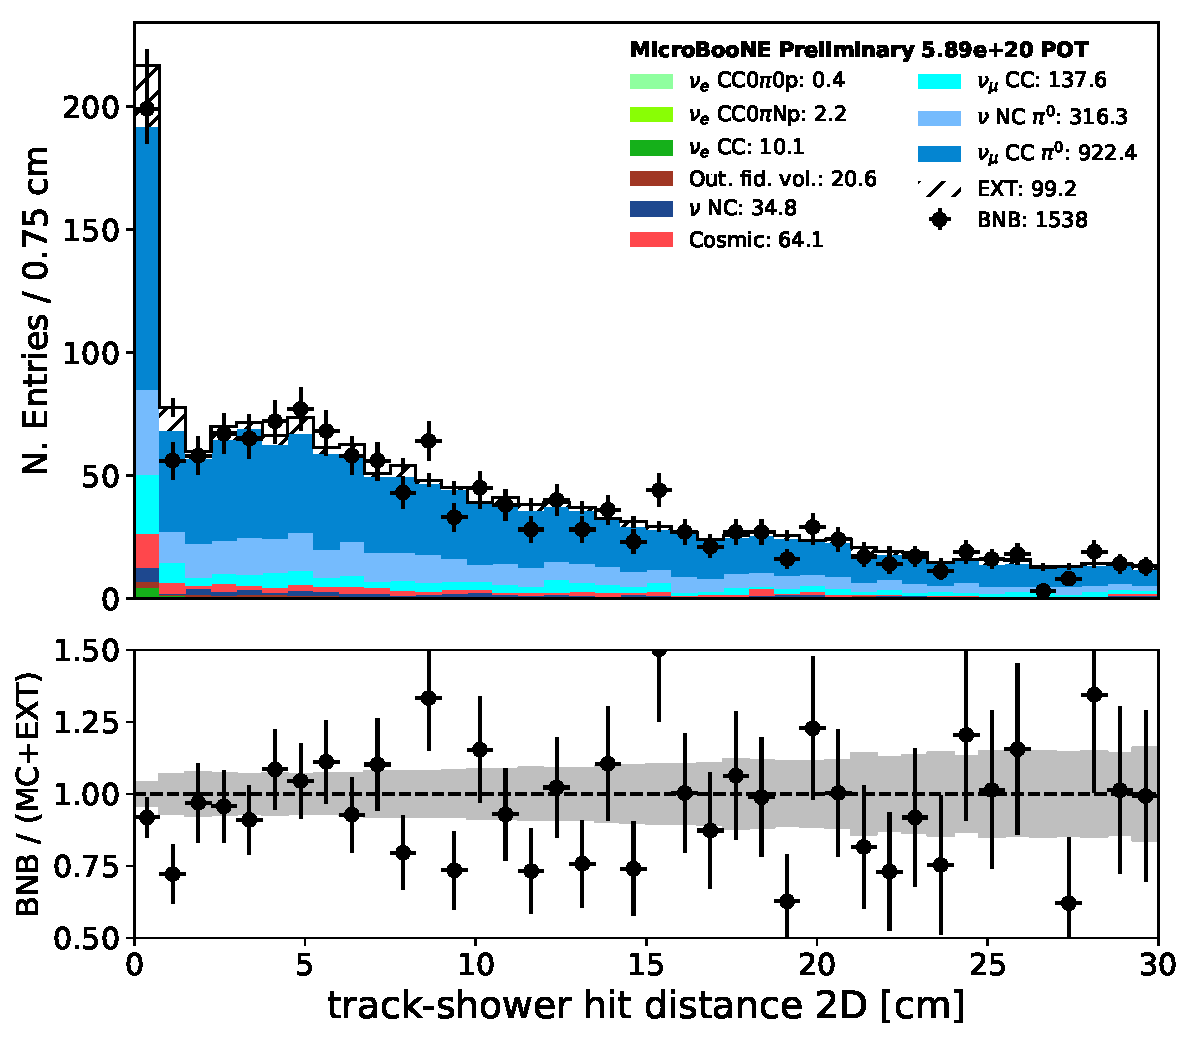
\includegraphics[width=1.00\textwidth]{pi0/nueselection/trkshrhitdist2_03112020_ALL_scaled.pdf}
    \caption{}
    \end{subfigure}
    \begin{subfigure}[b]{0.3\textwidth}
    \centering
    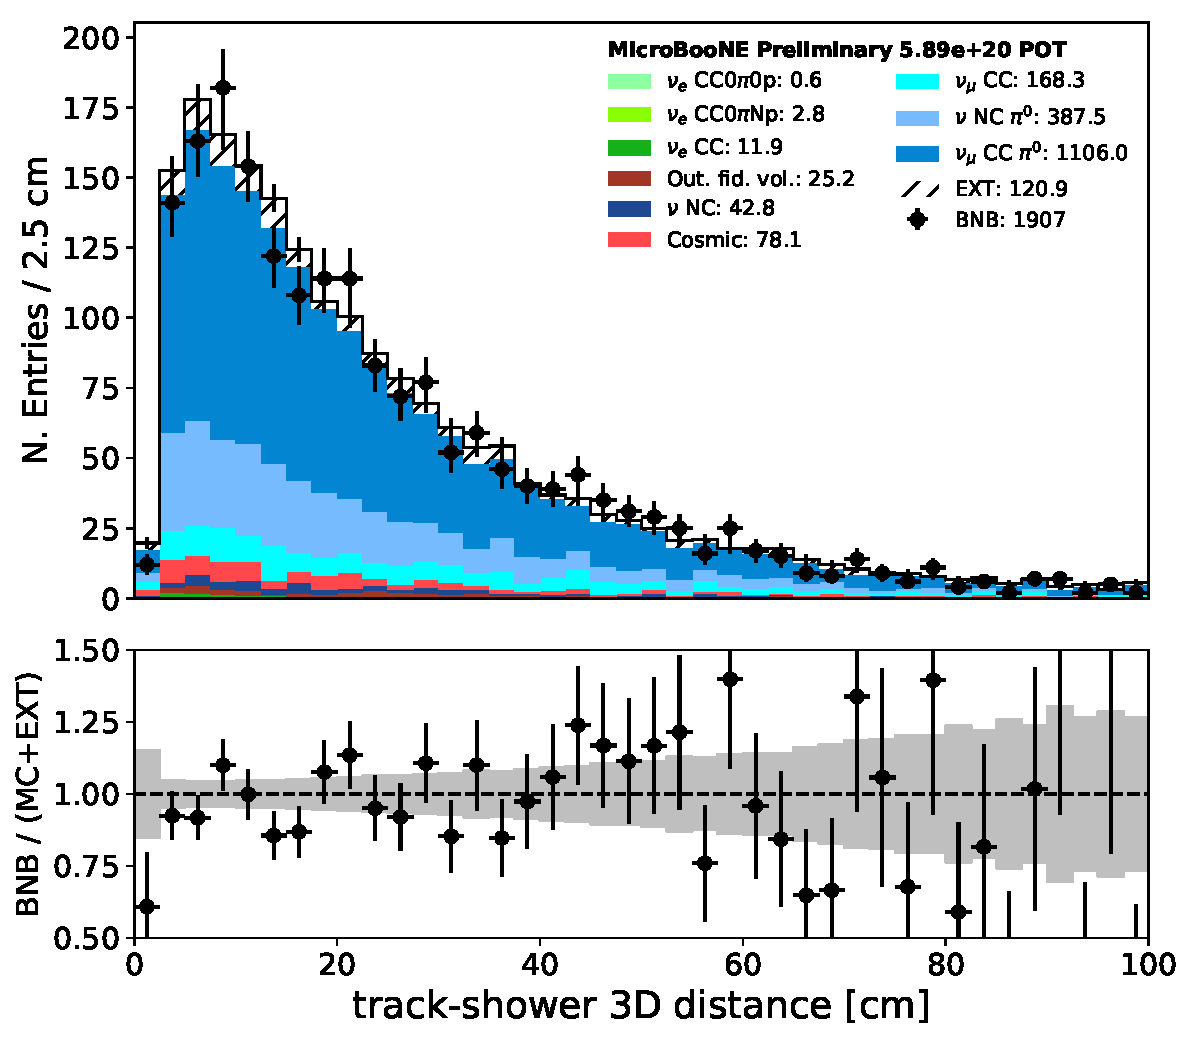
\includegraphics[width=1.00\textwidth]{pi0/nueselection/tksh_distance_03112020_ALL_scaled.pdf}
    \caption{}
    \end{subfigure}
    \begin{subfigure}[b]{0.3\textwidth}
    \centering
    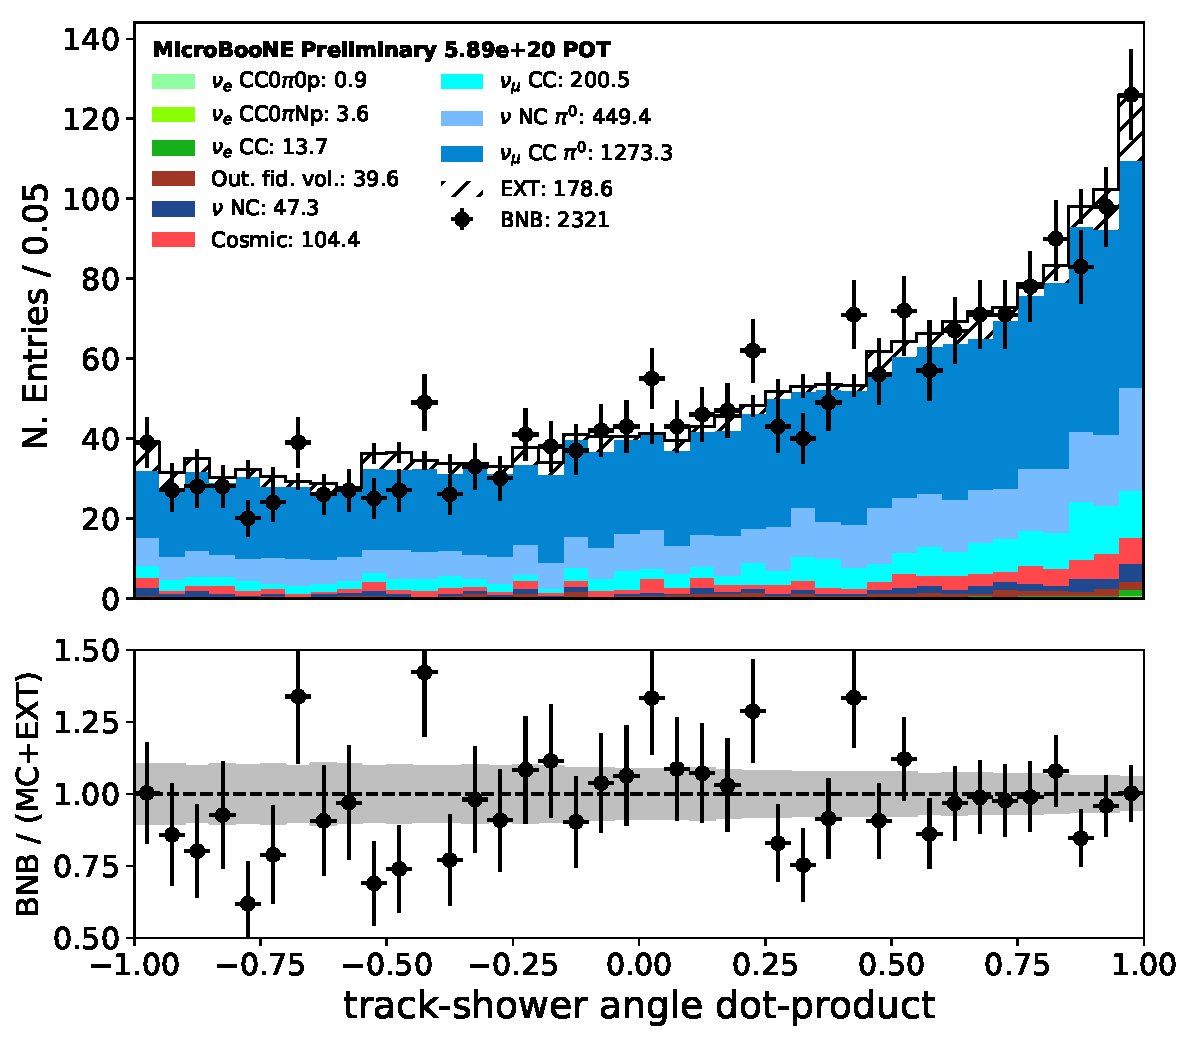
\includegraphics[width=1.00\textwidth]{pi0/nueselection/tksh_angle_03112020_ALL_scaled.pdf}
    \caption{}
    \end{subfigure}
\caption{}
\label{fig:pi0:nueselection:trkvar}
\end{center}
\end{figure}

\begin{figure}[H] 
\begin{center}
    \begin{subfigure}[b]{0.3\textwidth}
    \centering
    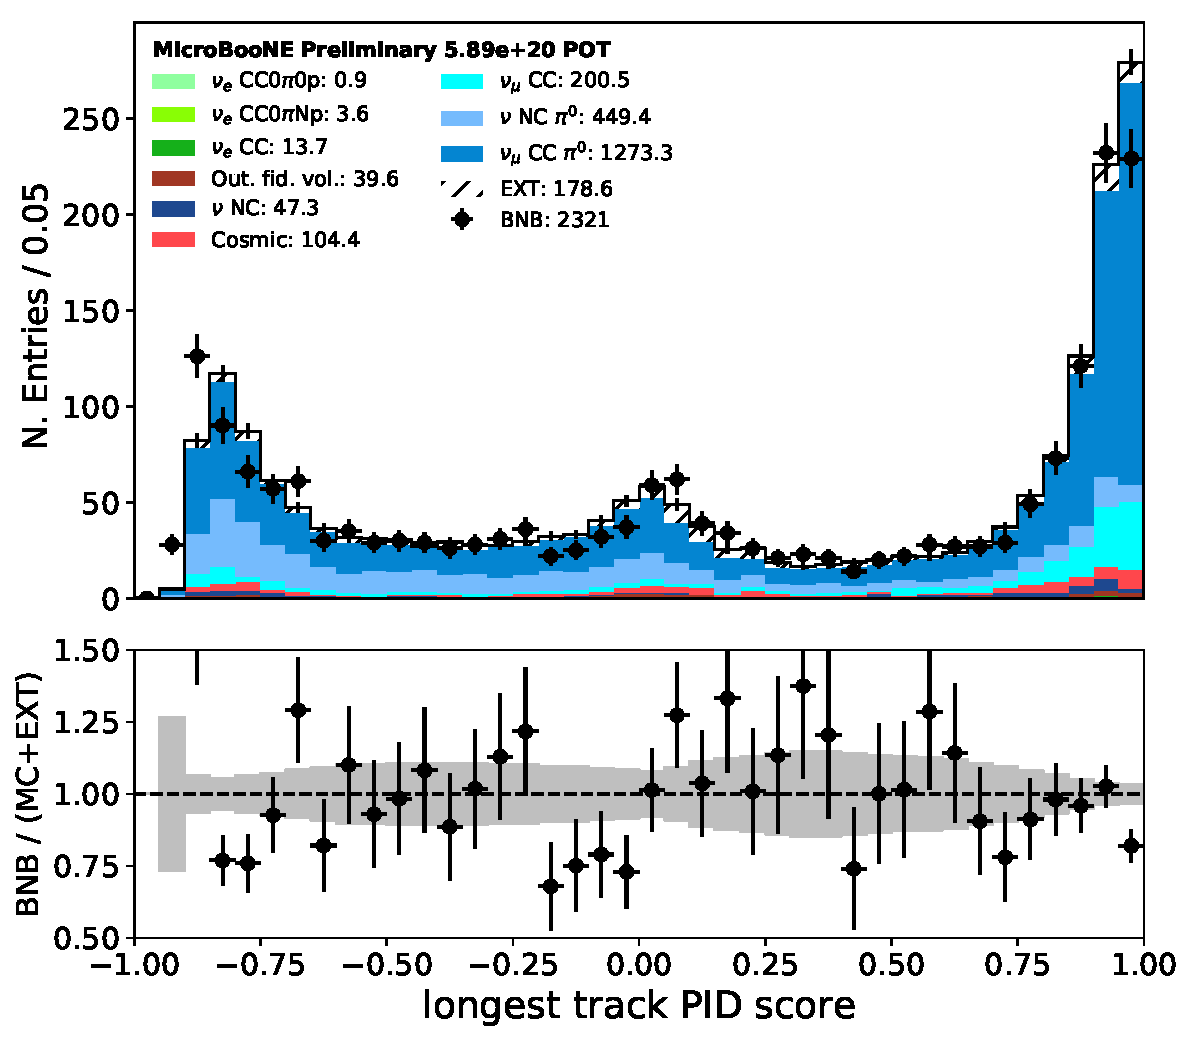
\includegraphics[width=1.00\textwidth]{pi0/nueselection/trkpid_03112020_ALL_scaled.pdf}
    \caption{}
    \end{subfigure}
    \begin{subfigure}[b]{0.3\textwidth}
    \centering
    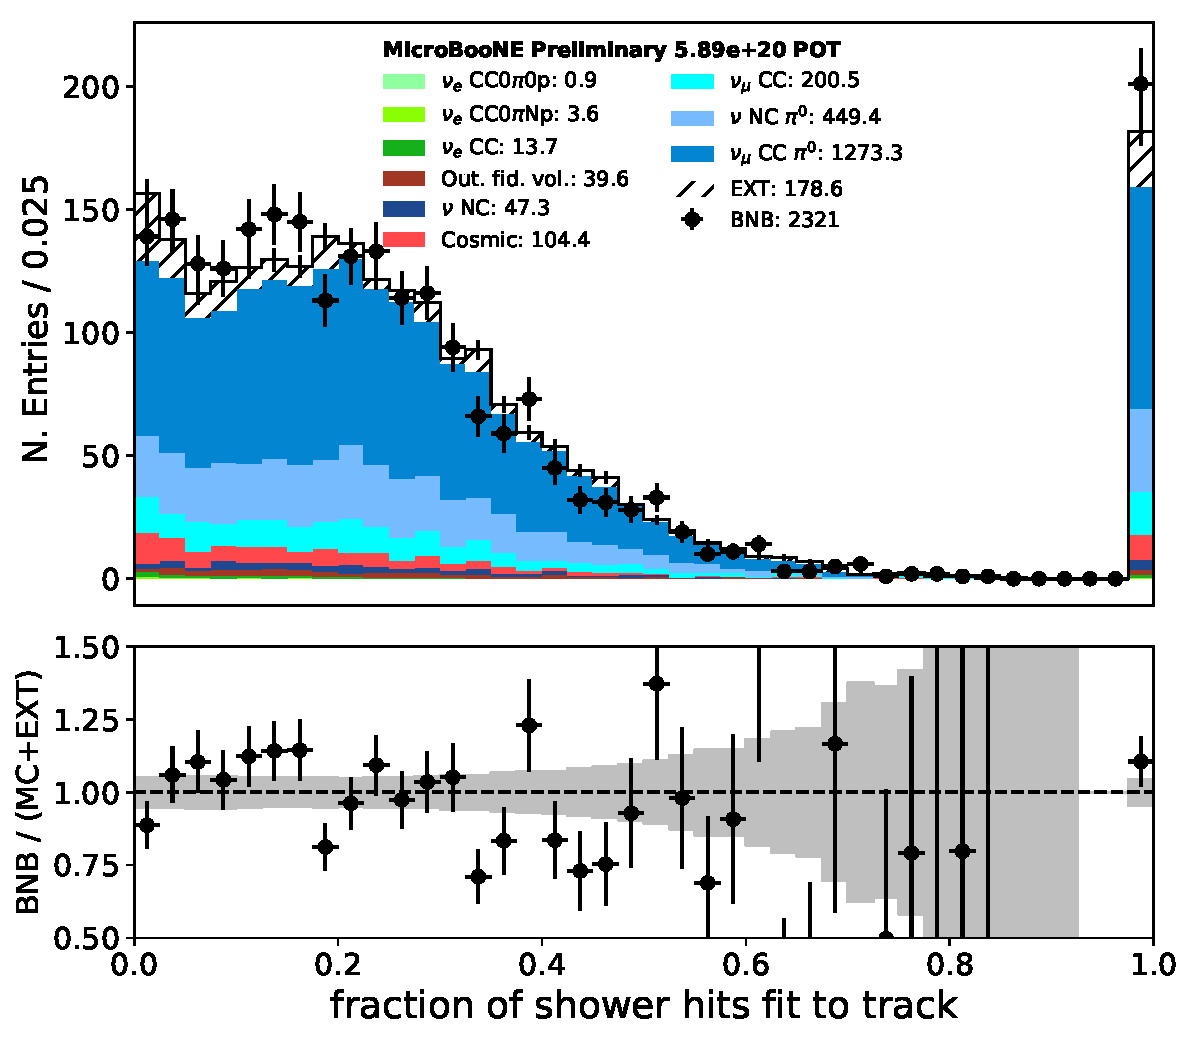
\includegraphics[width=1.00\textwidth]{pi0/nueselection/trkfit_03112020_ALL_scaled.pdf}
    \caption{}
    \end{subfigure}
    \begin{subfigure}[b]{0.3\textwidth}
    \centering
    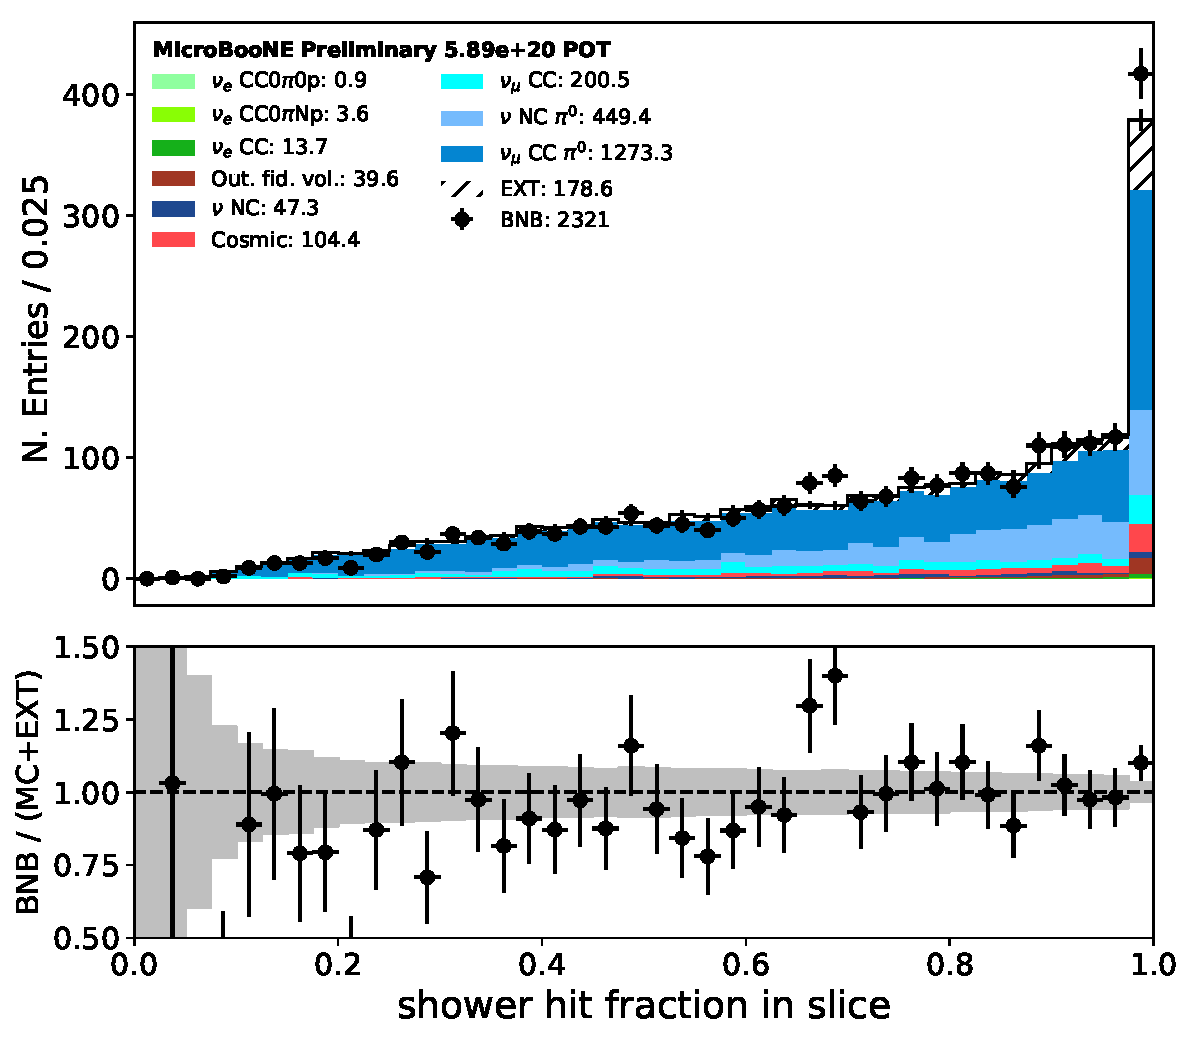
\includegraphics[width=1.00\textwidth]{pi0/nueselection/hits_ratio_03112020_ALL_scaled.pdf}
    \caption{}
    \end{subfigure}
\caption{}
\label{fig:pi0:nueselection:trkvar2}
\end{center}
\end{figure}

\begin{figure}[H] 
\begin{center}
    \begin{subfigure}[b]{0.3\textwidth}
    \centering
    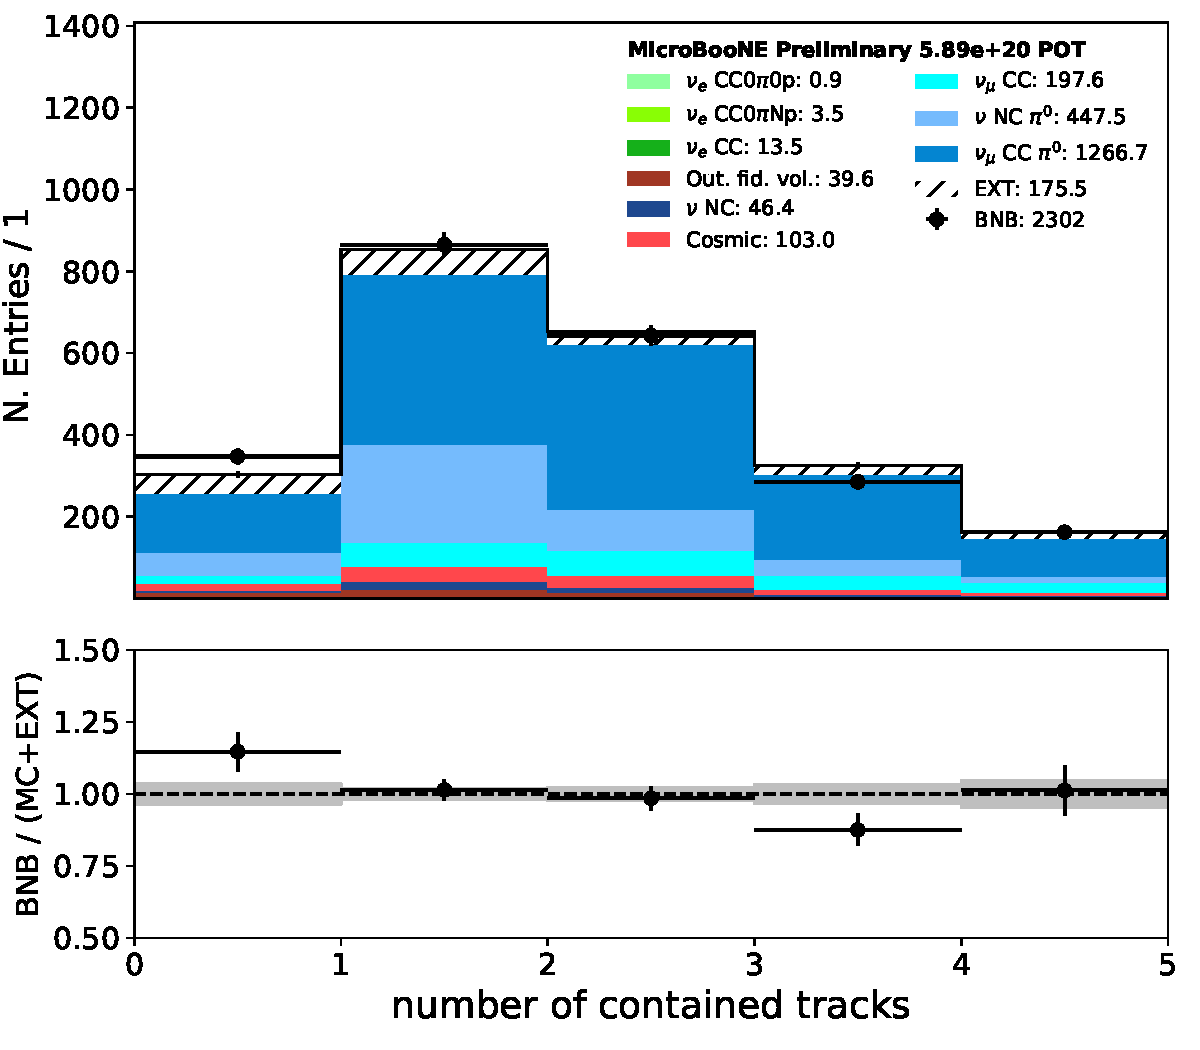
\includegraphics[width=1.00\textwidth]{pi0/nueselection/n_tracks_contained_03112020_ALL_scaled.pdf}
    \caption{}
    \end{subfigure}
    \begin{subfigure}[b]{0.3\textwidth}
    \centering
    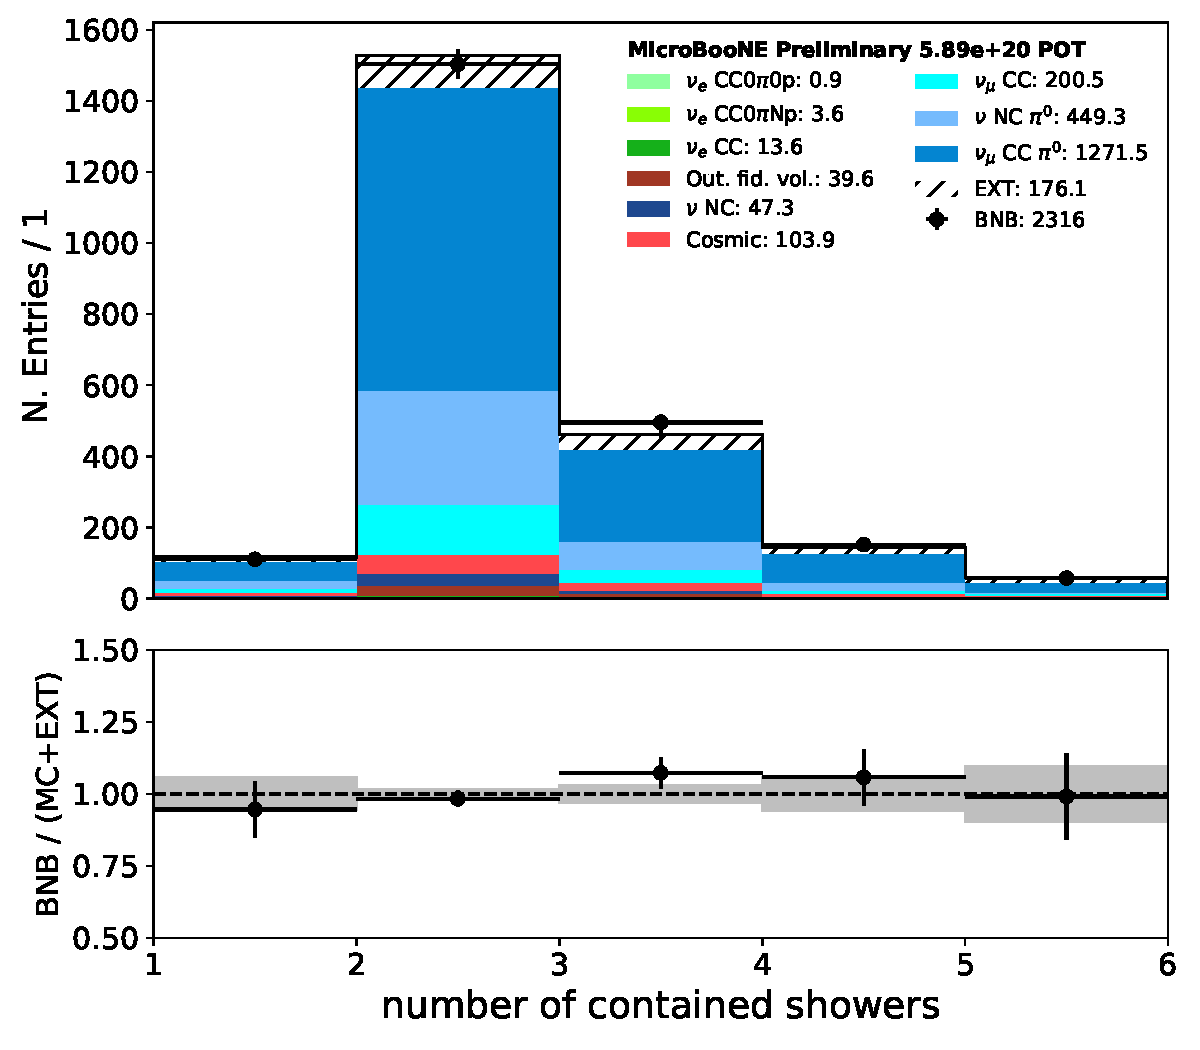
\includegraphics[width=1.00\textwidth]{pi0/nueselection/n_showers_contained_03112020_ALL_scaled.pdf}
    \caption{}
    \end{subfigure}
    \begin{subfigure}[b]{0.3\textwidth}
    \centering
    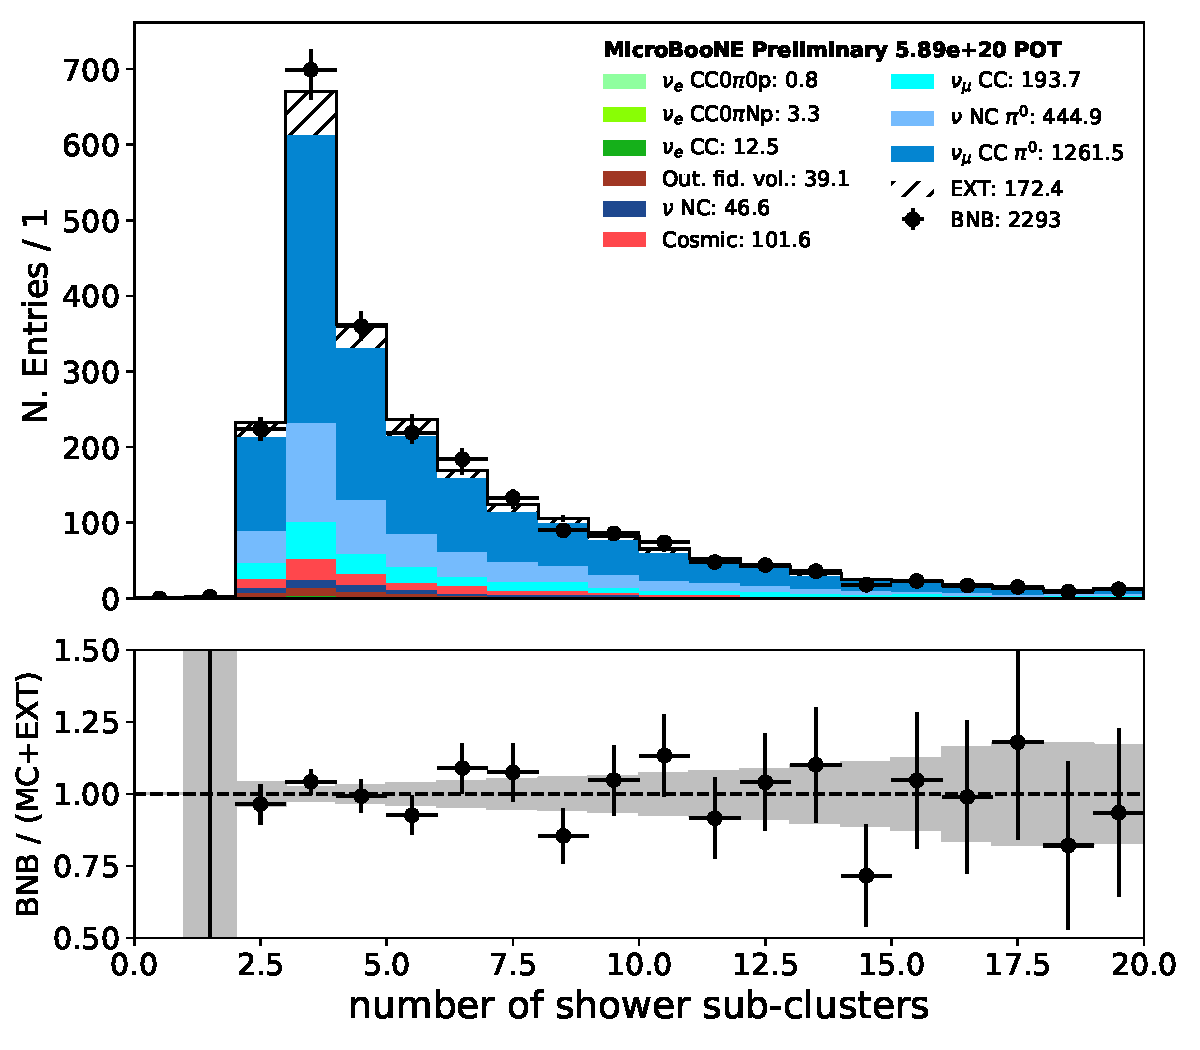
\includegraphics[width=1.00\textwidth]{pi0/nueselection/subcluster_03112020_ALL_scaled.pdf}
    \caption{}
    \end{subfigure}
\caption{}
\label{fig:pi0:nueselection:trkvar2}
\end{center}
\end{figure}


\begin{figure}[H] 
\begin{center}
    \begin{subfigure}[b]{0.3\textwidth}
    \centering
    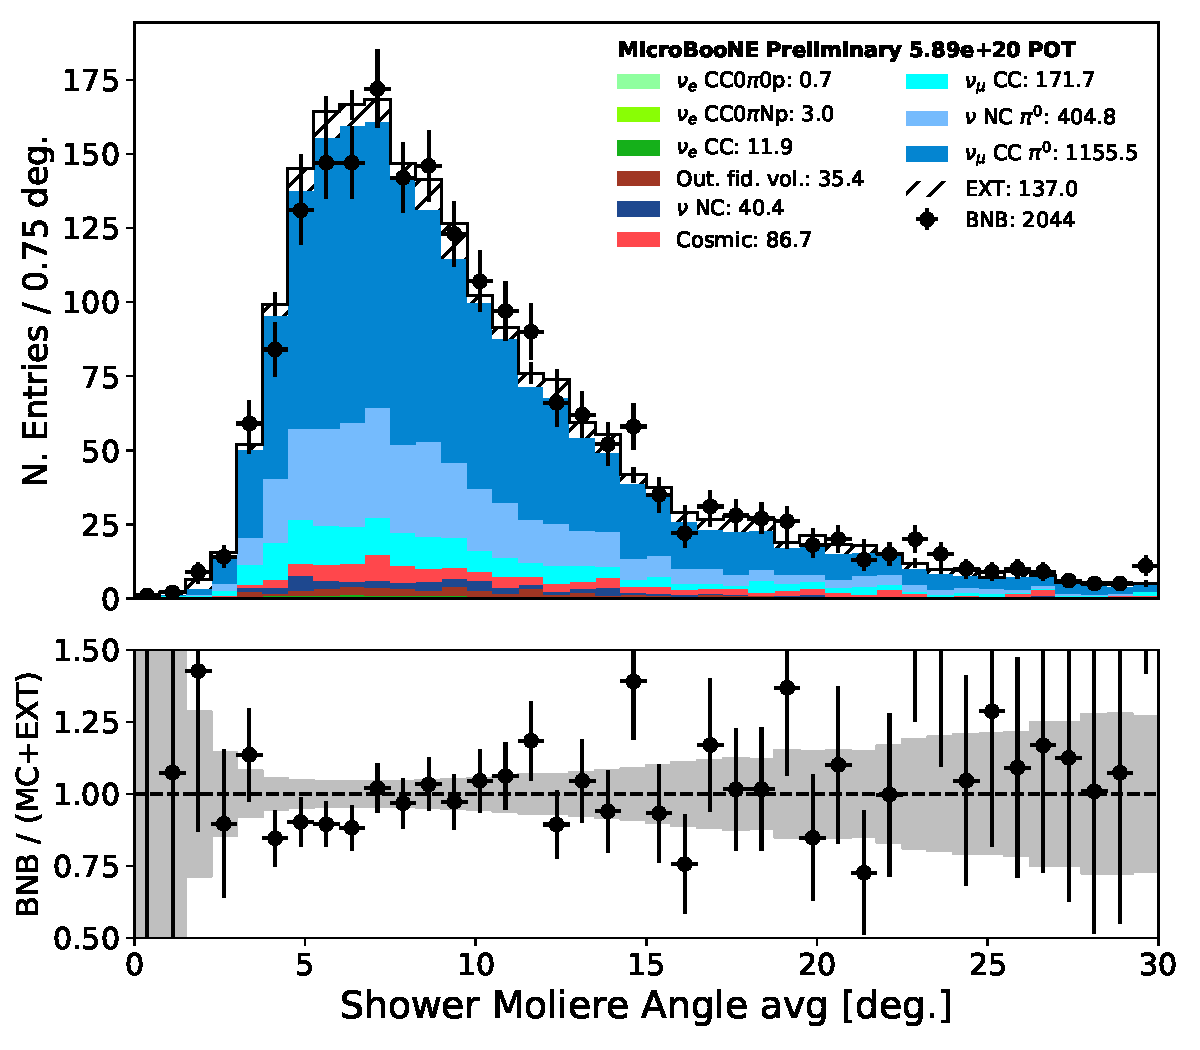
\includegraphics[width=1.00\textwidth]{pi0/nueselection/shrmoliereavg_03112020_ALL_scaled.pdf}
    \caption{}
    \end{subfigure}
    \begin{subfigure}[b]{0.3\textwidth}
    \centering
    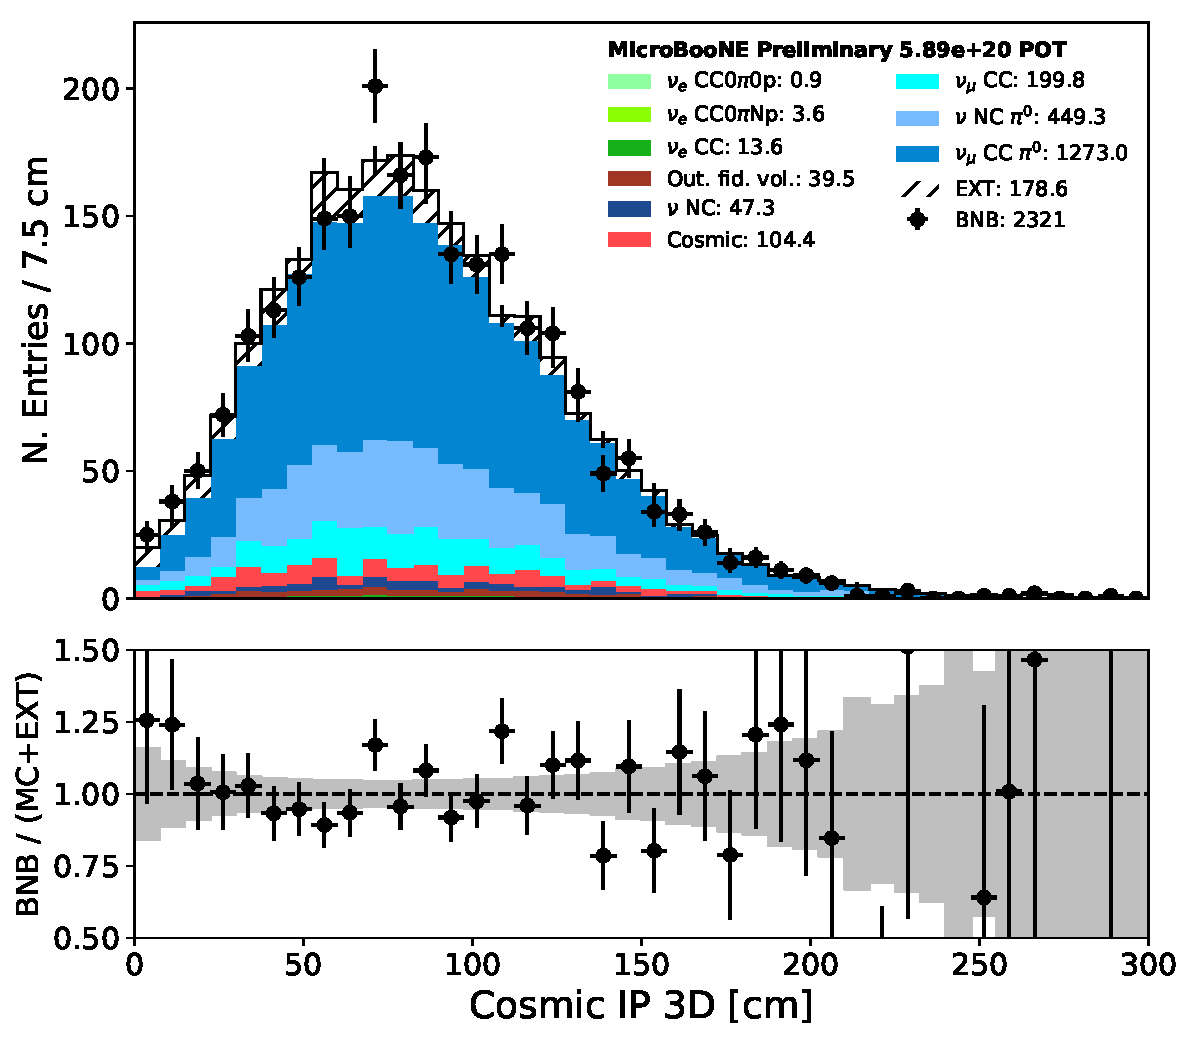
\includegraphics[width=1.00\textwidth]{pi0/nueselection/CosmicIPAll3D_03112020_ALL_scaled.pdf}
    \caption{}
    \end{subfigure}
\caption{}
\label{fig:pi0:nueselection:trkvar2}
\end{center}
\end{figure}